\documentclass{beamer}
\usepackage[section]{placeins}
\usepackage{float}
\usepackage[position=b]{subfig}
\usepackage{etoolbox}% http://ctan.org/pkg/etoolbox
\setbeamertemplate{caption}[numbered]
% \AtBeginEnvironment{figure}{\setcounter{subfigure}{0}}% Resets subfigure counter at start of figure environment

\mode<presentation>{
  %   \usetheme{CambridgeUS}      % or try Darmstadt, Madrid, Warsaw, ...
  \usetheme{Frankfurt}
  % \definecolor{mygreen}{cmyk}{0.6,0.168,0.168,0.25}
  % \definecolor{mygreen}{RGB}{84,135,138}

  % \definecolor{myblue}{RGB}{23, 91, 127}
  \definecolor{myblue}{RGB}{24, 71, 160}
  \setbeamercolor{structure}{fg=myblue}
  \usefonttheme{default}
  \setbeamertemplate{navigation symbols}{}
  %\setbeamertemplate[compatibility=false, numbered]{caption}
  \setbeamertemplate{itemize items}[default]
  \setbeamertemplate{enumerate items}[default]
  \defbeamertemplate*{title page}{customized}[1][]{
    \centering
      \begin{beamercolorbox}[rounded=true,shadow=true,leftskip=1cm,colsep*=.75ex]{title}
        \centering
          \usebeamerfont{title}\inserttitle\par
      \end{beamercolorbox}
      \par\medskip\medskip\medskip
      \begin{columns}
        \begin{column}{0.6\textwidth}
          \usebeamerfont{author}\insertauthor\par\medskip\medskip
          \usebeamerfont{institute}\insertinstitute\par\medskip\medskip
          \usebeamerfont{date}\insertdate\par
          % \medskip \medskip \medskip
          \begin{figure}[!htbp]
            \begin{center}
              \subfloat{
                
\includegraphics[width=0.4\columnwidth]{figuras/cnpqLogo.jpg}
              }
              \hspace{1cm}
              \subfloat{
                
\includegraphics[width=0.2\columnwidth]{figuras/capesLogo.png}
              }
            \end{center}
          \end{figure}
        \end{column}
        \begin{column}{0.3\textwidth}
          
\includegraphics[width=\columnwidth]{figuras/brasao_usp_pb}
        \end{column}
      \end{columns}
  }

  \setbeamertemplate{footline}{
    \begin{beamercolorbox}[colsep=1.5pt]{upper separation line foot}
    \end{beamercolorbox}
    \hbox{%
      \begin{beamercolorbox}[wd=0.82\paperwidth, ht=2.5ex, dp=1.125ex, left]{title in head/foot}%
        \usebeamerfont{title in head/foot}\hspace*{2ex}\insertshorttitle
      \end{beamercolorbox}%

      \begin{beamercolorbox}[wd=0.09\paperwidth, ht=2.5ex, dp=1.125ex, center]{title in head/foot}%
        \usebeamerfont{author in head/foot}{\insertshortinstitute }
      \end{beamercolorbox}%

      \begin{beamercolorbox}[wd=0.09\paperwidth, ht=2.5ex, dp=1.125ex, right]{title in head/foot}%
        \usebeamerfont{title in head/foot}\insertframenumber/\inserttotalframenumber\hspace*{2ex}
      \end{beamercolorbox}
    }
    \begin{beamercolorbox}[colsep=1.5pt]{lower separation line foot}
    \end{beamercolorbox}
  }
}

\makeatletter
\renewcommand{\itemize}[1][]{%
  \beamer@ifempty{#1}{}{\def\beamer@defaultospec{#1}}%
  \ifnum \@itemdepth >2\relax\@toodeep\else
    \advance\@itemdepth\@ne
    \beamer@computepref\@itemdepth% sets \beameritemnestingprefix
    \usebeamerfont{itemize/enumerate \beameritemnestingprefix body}%
    \usebeamercolor[fg]{itemize/enumerate \beameritemnestingprefix body}%
    \usebeamertemplate{itemize/enumerate \beameritemnestingprefix body begin}%
    \list
      {\usebeamertemplate{itemize \beameritemnestingprefix item}}
      {\def\makelabel##1{%
          {%
            \hss\llap{{%
                \usebeamerfont*{itemize \beameritemnestingprefix item}%
                \usebeamercolor[fg]{itemize \beameritemnestingprefix item}##1}}%
          }%
        }%
      }
  \fi%
  \beamer@cramped%
  \justifying% NEW
  %\raggedright% ORIGINAL
  \beamer@firstlineitemizeunskip%
}
\makeatother

\useoutertheme[subsection=false]{miniframes}
\usepackage{etoolbox}
\makeatletter
\patchcmd{\slideentry}{\advance\beamer@xpos by1\relax}{}{}{}
\def\beamer@subsectionentry#1#2#3#4#5{\advance\beamer@xpos by1\relax}%
\makeatother

\usepackage{ragged2e}
\usepackage{lipsum}
\usepackage[sort, numbers]{natbib}
% \usepackage[style=alphabetic]{biblatex}

\usepackage[linesnumbered,ruled,vlined]{algorithm2e}
%\usepackage{algorithm}
\usepackage{algpseudocode}
\SetKwFor{Para}{para}{fa\c{c}a}{fim}
\SetKwFor{ParaCada}{para cada}{fa\c{c}a}{fim}
\SetKwRepeat{DoWhile}{faça}{enquanto}

\usepackage[compatibility=false]{caption}
% \usepackage{subcaption}
\usepackage[brazil]{babel}
\usepackage[utf8x]{inputenc}
\usepackage{setspace}
\usepackage{ragged2e}
\usepackage{graphicx}
\usepackage{amsmath,amsfonts,amssymb}
\usepackage{xcolor}
\usepackage{url}
\usepackage{array}
\usepackage{gensymb}
\usepackage{multicol}
\usepackage[loadonly]{enumitem}
\newlist{arrowlist}{itemize}{1}
\setlist[arrowlist]{label=$\Rightarrow$}
\usepackage{listings}
\newcommand{\fonte}[1]{\caption*{Fonte: #1}}
\newcommand{\fonteminha}{\caption*{Fonte: Elaborado pelo autor.}}

\title[\textbf{Geração de imagens artificiais e quantização aplicadas a problemas de classificação}]{\textbf{Geração de imagens artificiais e quantização aplicadas a problemas de classificação}}
\author{Gabriela Salvador Thumé \\ \vspace{4pt}
        \tiny Orientador: Prof. Dr. Moacir Antonelli Ponti \\ \vspace{4pt}
        \tiny Co-orientador: Prof. Dr. João do Espirito Santo Batista Neto}
\institute[ICMC/USP]{Instituto de Ciências Matemáticas e de Computação \\
Universidade de São Paulo \\ }
\date{29 de abril de 2016}
%%%%%%%%%%%%%%%%%%%%%%%%%%%%%%%%%%%%%%%%%%%%%%%%%%%%%%%%%%%%%%%%%%%%%%%%%%%%%%%
\begin{document}
  \setbeamercovered{transparent}
  \begin{frame}[plain]
    \maketitle
\end{frame}
%%%%%%%%%%%%%%%%%%%%%%%%%%%%%%%%%%%%%%%%%%%%%%%%%%%%%%%%%%%%%%%%%%%%%%%%%%%%%%%
\begin{frame}[noframenumbering]{Estrutura da Apresentação}
  \setstretch{1.2}
  \setlength\leftmargini{1em}
  \begin{multicols}{2}
    \tableofcontents
  \end{multicols}
\end{frame}
%%%%%%%%%%%%%%%%%%%%%%%%%%%%%%%%%%%%%%%%%%%%%%%%%%%%%%%%%%%%%%%%%%%%%%%%%%%%%%%
\section{Introdução}
\AtBeginSection[]{
  \begin{frame}<beamer>[noframenumbering]{Estrutura da Apresentação}
    \setstretch{1.2}
    \setlength\leftmargini{1em}
    \begin{multicols}{2}
    \tableofcontents[currentsection, sectionstyle=show/shaded,
    ]
    % \tableofcontents[currentsection,currentsubsection, hideothersubsections,
    %     sectionstyle=show/shaded,
    % ]
    \end{multicols}
  \end{frame}
}
%%%%%%%%%%%%%%%%%%%%%%%%%%%%%%%%%%%%%%%%%%%%%%%%%%%%%%%%%%%%%%%%%%%%%%%%%%%%%%%
\begin{frame}{Introdução}
  \setstretch{1.2}
  \setlength\leftmargini{1em}
  \justifying
  \begin{itemize}
    \item Classificação de imagens: predizer a classe;
    \pause
    \item Extração de características: vetores representativos;
    \pause
    \item Algoritmos de aprendizado de máquina: modelo de representação;
    \pause
    \item Generalização: classificar novos exemplos;
    \pause
    \item Porém, existem características que não são suficientes para a diferenciação entre as classes;
    % \item Encontrar as características que melhor discriminam as classes.
  \end{itemize}
\end{frame}
%-----------------------------------------------------------------------------
\subsection{Motivação}
\begin{frame}{Motivação}
  \setstretch{1.2}
  \setlength\leftmargini{1em}
  \justifying
  \begin{itemize}
    \item Maior esforço ao operar no espaço de características já obtidas;
    \item Transformações do espaço ou sistemas complexos de classificação para lidar com as deficiências das características extraídas;
    \item Características que podem ser exploradas além dos métodos clássicos;
    \item Investigar métodos de \textit{processamento e preparação de imagens antes da extração}.
  \end{itemize}
\end{frame}
%-----------------------------------------------------------------------------
\begin{frame}[plain]{Motivação}
  \setstretch{1.2}
  \setlength\leftmargini{1em}
  \begin{figure}
    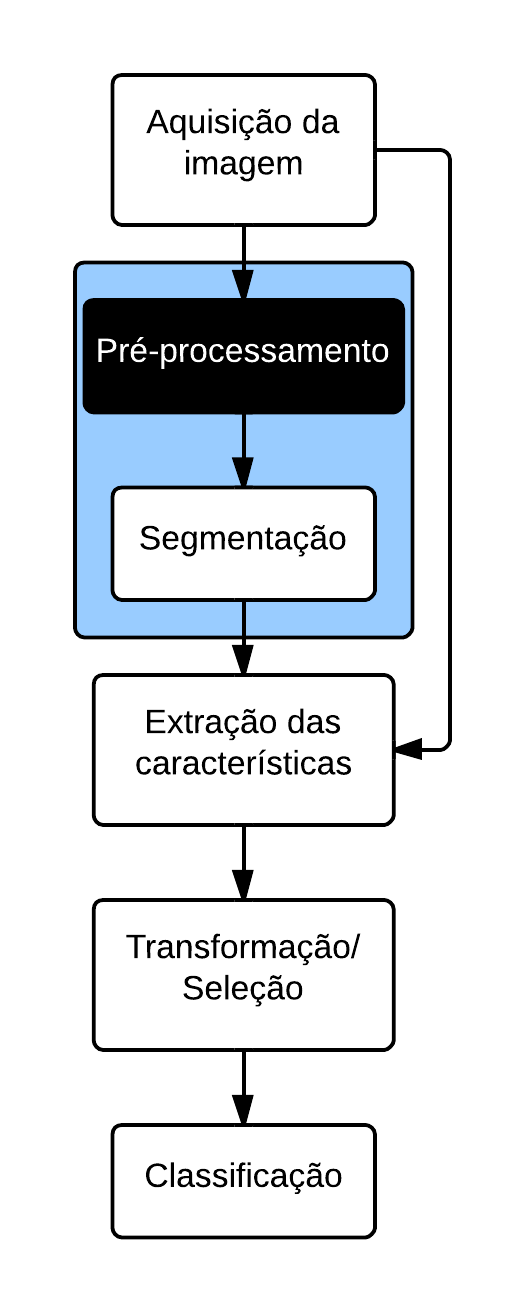
\includegraphics[height=0.9\textheight]{figuras/flow.png}
    \caption{Etapas canônicas do reconhecimento de padrões.}
  \end{figure}
\end{frame}
%-----------------------------------------------------------------------------
% \begin{frame}{Motivação --- Características Latentes}
%   \setstretch{1.2}
%   \setlength\leftmargini{1em}
%   \justifying
%   \setstretch{1.2}
%   \begin{itemize}
%     \item Justificado o uso de métodos de processamento e preparação de imagens antes da extração;
%     \item Podem revelar características latentes, que possam melhor descrever certas classes, utilizando algoritmos sobre as imagens originais.
%   \end{itemize}
% \end{frame}
%-----------------------------------------------------------------------------
\begin{frame}{Motivação --- Quantização}
  \setstretch{1.2}
  \setlength\leftmargini{1em}
  \justifying
  \setstretch{1.2}
  \begin{itemize}
    \justifying
    \item Redução da complexidade no ínicio do reconhecimento;
    \item Apesar de fazer parte do pipeline, muitos estudos não descrevem o método de quantização e seus parâmetros;
    \item Quantização pode impactar a classificação (Kanan e Cottrell, 2012);
    \item Ao negligenciar essa etapa, perde-se a \textit{oportunidade de redução da dimensionalidade do vetor de características e/ou do tempo de execução das etapas posteriores.}
  \end{itemize}
\end{frame}
%-----------------------------------------------------------------------------
\begin{frame}{Motivação --- Desbalanceamento de classes}
  \setstretch{1.2}
  \setlength\leftmargini{1em}
  \justifying
  \setstretch{1.2}
  \begin{itemize}
    \item Diferença entre o número de exemplos disponíveis;
    \item Imagens representam eventos importantes mas menos frequentes;
    \item Métodos de transformação do espaço e de
    classificação assumem que a base está balanceada;
    \item Preferência à predição da classe majoritária, prejudicando a classificação da minoritária.
  \end{itemize}
\end{frame}
%-----------------------------------------------------------------------------
\begin{frame}{Motivação --- Rebalanceamento de classes}
  \setstretch{1.2}
  \setlength\leftmargini{1em}
  \justifying
  % \setstretch{1.2}
  \begin{itemize}
    \item Synthetic Minority Over-sampling Technique (SMOTE) propõe a geração de exemplos a partir dos vetores de características originais das classes minoritárias;
    \item Não existem estudos dessas técnicas em dados de informação visual para o rebalanceamento de classes;
    \item Proposta: \textit{geração de imagens artificiais a partir do processamento das imagens da classe minoritária.}
  \end{itemize}
  \begin{figure}[htbp]
    \begin{center}
      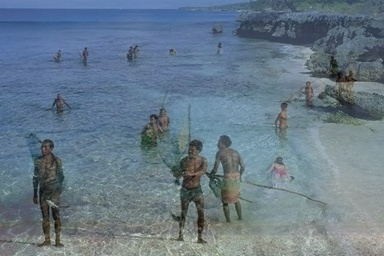
\includegraphics[width=.35\linewidth]{figuras/imagemgerada.jpg}
      \caption{Imagem artificialmente gerada.}
    \end{center}
  \end{figure}
\end{frame}
%-----------------------------------------------------------------------------
\subsection{Hipóteses}
\setstretch{1.2}
\setlength\leftmargini{1em}
\justifying
\begin{frame}{Hipóteses}
  \begin{block}{Utilizar um número reduzido de cores}
    \justifying
    \begin{itemize}
      \item Juntamente com um método de quantização apropriado;
      \item Antes da extração de características;
      \item \textit{Obter vetores de características mais compactos e com maior capacidade de discriminação entre classes.}
    \end{itemize}
  \end{block}
  \begin{block}{Geração de imagens artificiais}
    \justifying
    \begin{itemize}
      \item Balancear as classes;
      \item Preparação para a extração de características;
      \item \textit{Melhorar a acurácia, quando comparada à geração de exemplos artificiais no espaço de atributos.}
    \end{itemize}
  \end{block}
\end{frame}
%%%%%%%%%%%%%%%%%%%%%%%%%%%%%%%%%%%%%%%%%%%%%%%%%%%%%%%%%%%%%%%%%%%%%%%%%%%%%%%
\subsection{Contribuições}
% \begin{frame}{Contribuição geral}
%   \setstretch{1.2}
%   \setlength\leftmargini{1em}
%   \justifying
%   \begin{block}{}
%     \justifying
%     \emph{Investigar os métodos de pré-processamento para preparar uma coleção de imagens para a extração de características.}
%
%     \vspace{5mm}
%     Observa-se o efeito da quantização de imagens e do balanceamento do número de instâncias de diferentes classes na classificação.
%   \end{block}
% \end{frame}
%-----------------------------------------------------------------------------
\begin{frame}{Contribuições}
  \setstretch{1.2}
  \setlength\leftmargini{1em}
  \justifying
  \begin{itemize}
    \item Demostrar que é possível obter vetores de características compactos e efetivos ao extrair características de imagens quantizadas.
    \begin{itemize}
      \item Custo computacional baixo;
      \item Reduzindo a dimensionalidade do vetor após a quantização e posterior extração de características;
      \item Redução do tempo de processamento para os métodos de descrição de textura.
    \end{itemize}
  \end{itemize}
\end{frame}
%-----------------------------------------------------------------------------
\begin{frame}{Contribuições}
  \setstretch{1.2}
  \setlength\leftmargini{1em}
  \justifying
  \begin{itemize}
    \item Demostrar que a geração de imagens artificiais pode contribuir com o balanceamento entre classes.
    \begin{itemize}
      \item Melhorando o \textit{F1-Score} resultante de algoritmos de classificação;
      \item Comparando com a geração de exemplos artificiais no espaço de atributos (SMOTE).
    \end{itemize}
  \end{itemize}
\end{frame}
%-----------------------------------------------------------------------------
\begin{frame}{Contribuições em código e reprodutibilidade}
  \setstretch{1.2}
  \setlength\leftmargini{1em}
  \justifying
  \begin{itemize}
    \item Código para a quantização:
    \begin{center}
      \small{\url{http://dx.doi.org/10.5281/zenodo.15932}}
    \end{center}
    \item Código da geração de imagens artificiais:
    \begin{center}
      \small{\url{https://github.com/GabiThume/msc-src}}
    \end{center}
  \end{itemize}
\end{frame}
%%%%%%%%%%%%%%%%%%%%%%%%%%%%%%%%%%%%%%%%%%%%%%%%%%%%%%%%%%%%%%%%%%%%%%%%%%%%%%%
% \subsection{Extração de características}
% \begin{frame}{Extração de Características}
% \setlength\leftmargini{0em}
% \justifying
% \begin{itemize}
% \item Descrever as informações visuais relevantes em um vetor de características;
% \item Entrada para o classificador de padrões;
% % Exemplo: importante para a discriminação entre classes de algas é a forma.
% \item Salientar as diferenças entre imagens de classes distintas e suavizar possíveis diferenças de imagens da mesma classe (Ex. algas - forma).
% \end{itemize}
% \setlength\leftmargini{0em}
% \begin{description}
% \item [Textura:] suavidade, aspereza e uniformidade. Ex. entropia;
% \item [Forma:] características externas. Ex. curvatura;\usepackage{etoolbox}% http://ctan.org/pkg/etoolbox
% Resets subfigure counter at start of figure environment
% \item [Cor:] distribuição espacial de cores na imagem. Ex. histograma.
% \end{description}
% \end{frame}
%%%%%%%%%%%%%%%%%%%%%%%%%%%%%%%%%%%%%%%%%%%%%%%%%%%%%%%%%%%%%%%%%%%%%%%%%%%%%%%
\section{Quantização de imagens}
\begin{frame}{Quantização de imagens}
  \setstretch{1.2}
  \setlength\leftmargini{1em}
  \begin{block}{}
    \justifying
    \begin{itemize}
      \item Métodos de extração preparados para receber imagens em um canal de cor;
      \item Características extraídas para cada canal de cor e posteriormente concatenadas;
      \item O pipeline de reconhecimento de imagens inclui a conversão de imagens coloridas em imagens com apenas um canal ($2^3$ = 8 bits);
      \item Explorar essa etapa para produzir vetores mais compactos;
      \item Diferentes parâmetros de quantização combinados com quatro métodos de extração de cor e um de textura.
    \end{itemize}
  \end{block}
\end{frame}

\subsection{Contextualização}
%-----------------------------------------------------------------------------
\begin{frame}{Pré-processamento de Imagens --- Quantização}
  \setstretch{1.2}
  \setlength\leftmargini{1em}
  \begin{figure}
    \begin{center}
      \subfloat[Original]{
      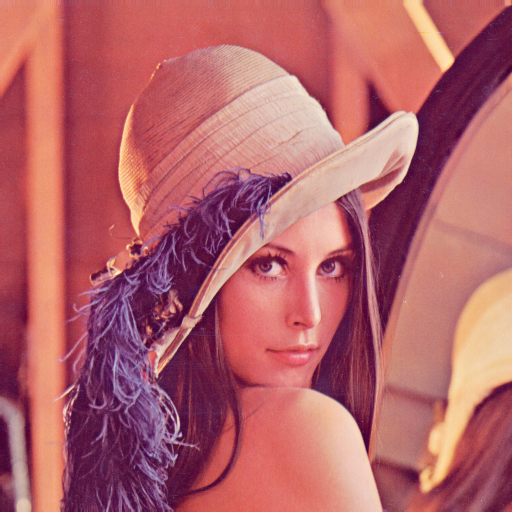
\includegraphics[width=.2\linewidth]{\detokenize{figuras/quantization/Lenna.png}}
      }
      \subfloat[Intensidade']{
      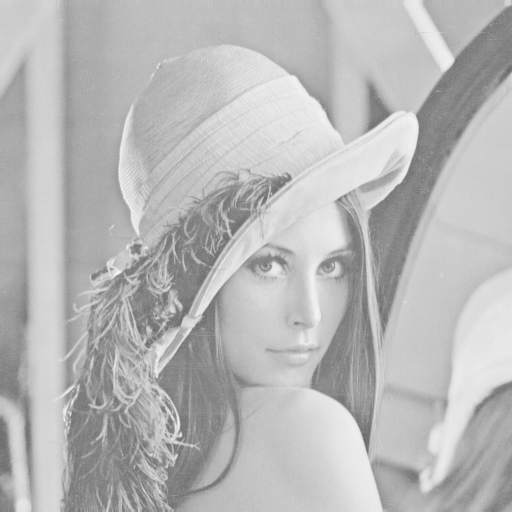
\includegraphics[width=.2\linewidth]{\detokenize{figuras/quantization/Intensity_gray.png}}
      }
      \subfloat[Gleam]{
      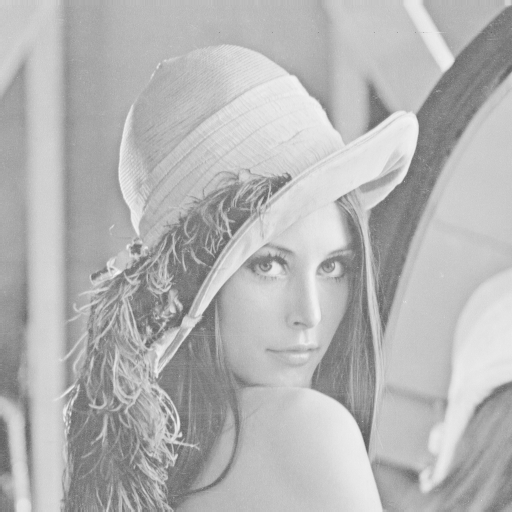
\includegraphics[width=.2\linewidth]{\detokenize{figuras/quantization/Gleam_gray.png}}
      }
    \end{center}
    \begin{center}
      \subfloat[Luminância']{
      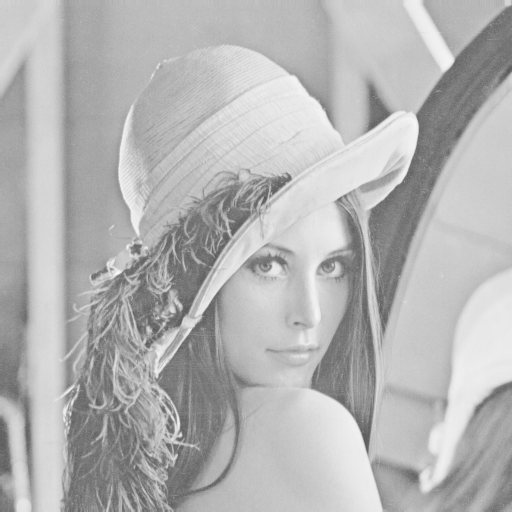
\includegraphics[width=.2\linewidth]{\detokenize{figuras/quantization/Luminance_gray.png}}
      }
      % \subfloat[Luma]{
      % 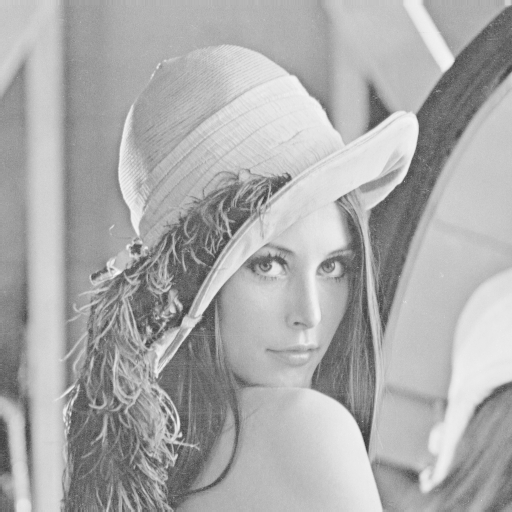
\includegraphics[width=.2\linewidth]{\detokenize{figuras/quantization/Luma_gray.png}}
      % }
      \subfloat[MSB]{
      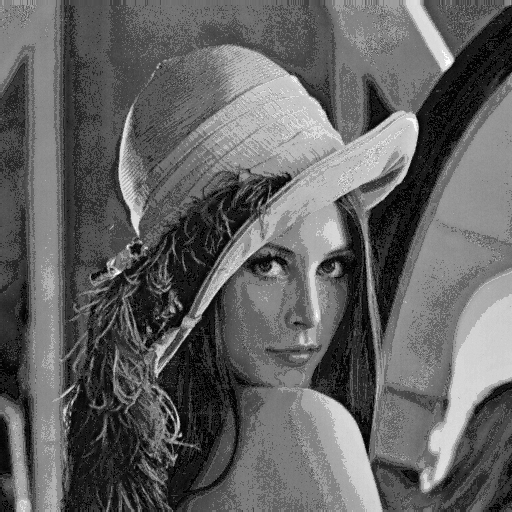
\includegraphics[width=.2\linewidth]{\detokenize{figuras/quantization/MSB_gray.png}}
      }
    \end{center}
    \caption{Conversão para a escala de cinza.}
  \end{figure}
\end{frame}
%-----------------------------------------------------------------------------
\begin{frame}{Quantização de imagens}
  \setstretch{1.2}
  \setlength\leftmargini{1em}
  \begin{figure}
    \begin{center}
      \centering
      \subfloat[Original]{
      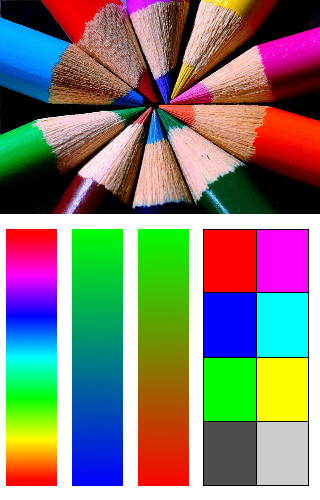
\includegraphics[width=.2\linewidth]{\detokenize{figuras/quantization/fig_quanttest.png}}
      }
      \subfloat[Gleam]{
      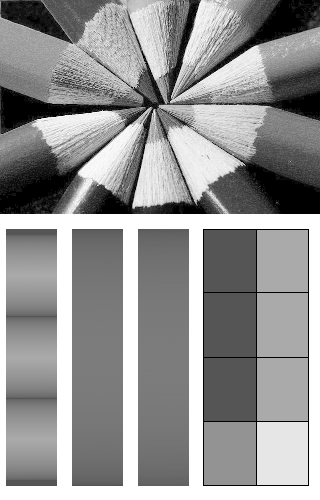
\includegraphics[width=.2\linewidth]{\detokenize{figuras/quantization/fig_quantGleam.png}}
      }
      \subfloat[Intensidade']{
      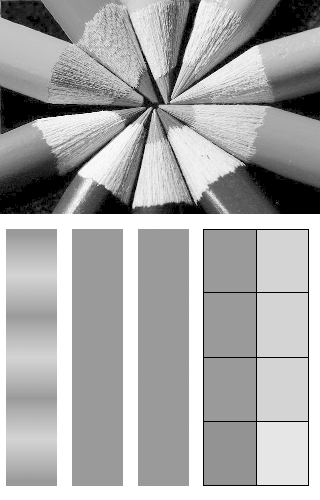
\includegraphics[width=.2\linewidth]{\detokenize{figuras/quantization/fig_quantIntensity.png}}
      }
      \subfloat[Luminância']{
      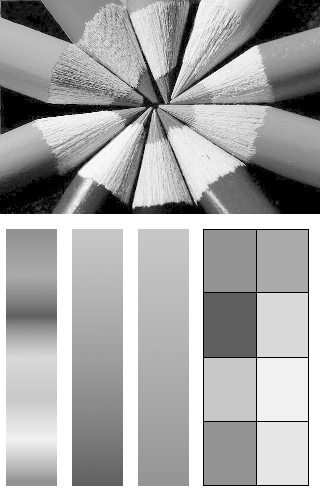
\includegraphics[width=.2\linewidth]{\detokenize{figuras/quantization/fig_quantLuminance.png}}
      }
      \subfloat[MSB]{
      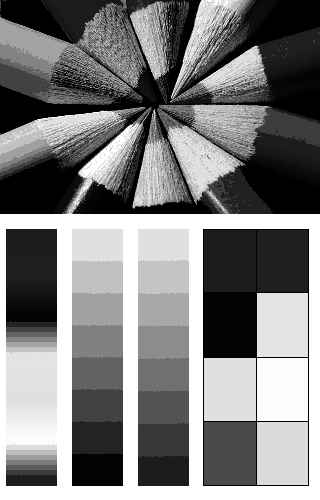
\includegraphics[width=.2\linewidth]{\detokenize{figuras/quantization/fig_quantMSB.png}}
      }
    \end{center}
    \caption{Os métodos \emph{Luminância'} e MSB apresentam uma melhor discriminação entre cores. A versão de um canal de cor possui 232 intensidades únicas para o método (e) MSB e 184 intensidades para os demais métodos.}
  \end{figure}
\end{frame}
%-----------------------------------------------------------------------------
\begin{frame}{Quantização de imagens}
  \setstretch{1.2}
  \setlength\leftmargini{1em}
  \begin{figure}
    \begin{center}
      \centering
      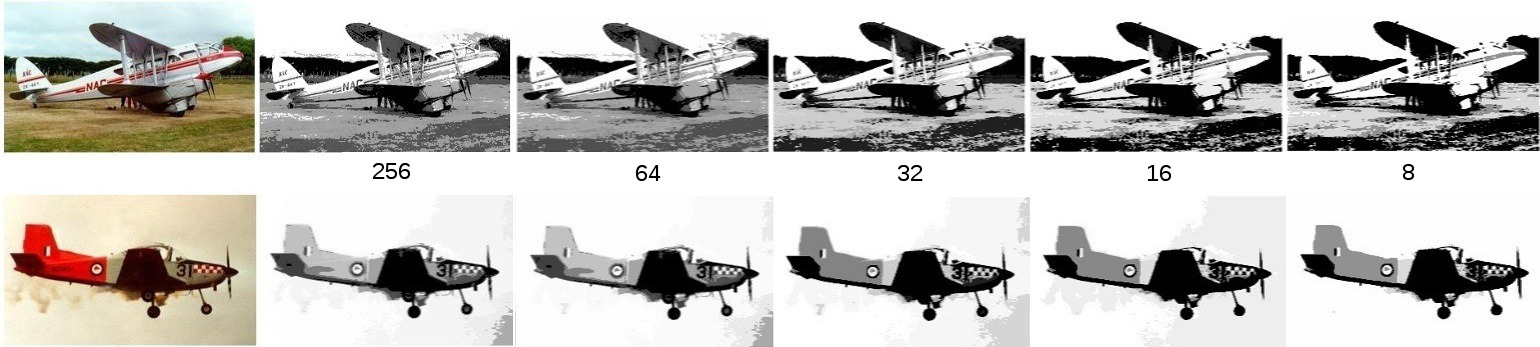
\includegraphics[width=\linewidth]{\detokenize{figuras/quantization/fig_quantizationexample.jpg}}
    \end{center}
    \caption{Imagens da base \emph{Caltech101-600} com variações no parâmetro de cor utilizando o método MSB. Com 256 e 64 há preservação das cores. Mas com apenas 32, há perda considerável de informação nas regiões com pouco contraste.}
  \end{figure}
\end{frame}
%%%%%%%%%%%%%%%%%%%%%%%%%%%%%%%%%%%%%%%%%%%%%%%%%%%%%%%%%%%%%%%%%%%%%%%%%%%%%%%
\subsection{Método}
%%%%%%%%%%%%%%%%%%%%%%%%%%%%%%%%%%%%%%%%%%%%%%%%%%%%%%%%%%%%%%%%%%%%%%%%%%%%%%%
\subsection{Experimentos}
\begin{frame}{Experimentos}
  \setstretch{1.2}
  \setlength\leftmargini{1em}
  \begin{block}{}
    \justifying
    \begin{itemize}
      \item Experimentos utilizando um método de extração de características seguido pela classificação (sem posterior seleção de características);
      \item Experimentos utilizando o vetor resultante da concatenação de todos os métodos de extração, seguido pela classificação com e sem a seleção de características.
    \end{itemize}
  \end{block}
\end{frame}
%-----------------------------------------------------------------------------
\begin{frame}{Experimentos}
  \setlength\leftmargini{1em}
  \begin{figure}
    \begin{center}
      \centering
      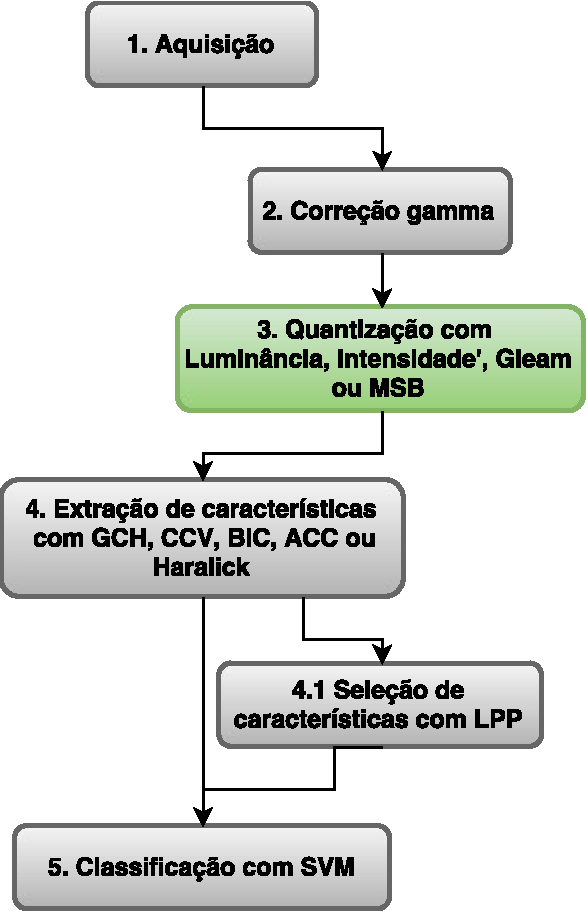
\includegraphics[width=0.4\linewidth]{\detokenize{figuras/quantization/quantizationResult.pdf}}
    \end{center}
    \caption{Fluxo das operações e os métodos utilizados nos experimentos.}
    %  Após a aquisição da imagem, ela é convertida para escala de cinza e seus níveis de cor são reduzidos de acordo com um parâmetro da quantização (i.e.\ número de cores). Dependendo do método, a correção \emph{gamma} é realizada. A imagem quantizada serve então como entrada para um método de extração de características e posteriormente é classificada com \emph{SVM}. Uma das etapas de experimentos prevê também a concatenação de todos os vetores extraídos e a seleção das características com \emph{LPP} antes da classificação.}
    \label{fig:quant:flowResult}
  \end{figure}
\end{frame}
%-----------------------------------------------------------------------------
\begin{frame}{Experimentos --- Bases de Imagens}
  \setlength\leftmargini{1em}
  \begin{figure}[!htbp]
    \begin{center}
      \begin{minipage}{.5\linewidth}
        \centering
        \subfloat[Corel-1000]{
          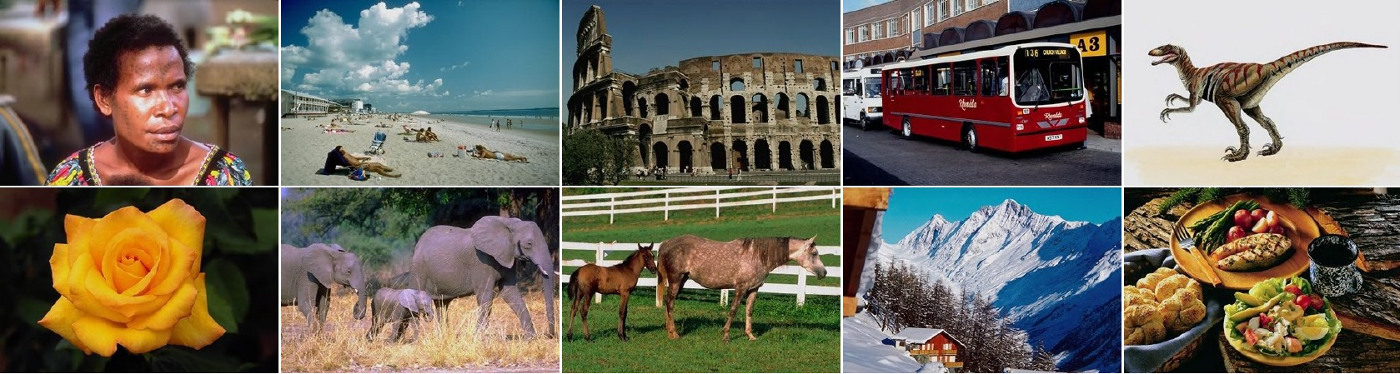
\includegraphics[width=.8\linewidth]{\detokenize{figuras/quantization/fig_COREL_dataset.jpg}}
        }
      \end{minipage}%
      \begin{minipage}{.5\linewidth}
        \subfloat[Caltech101-600]{
          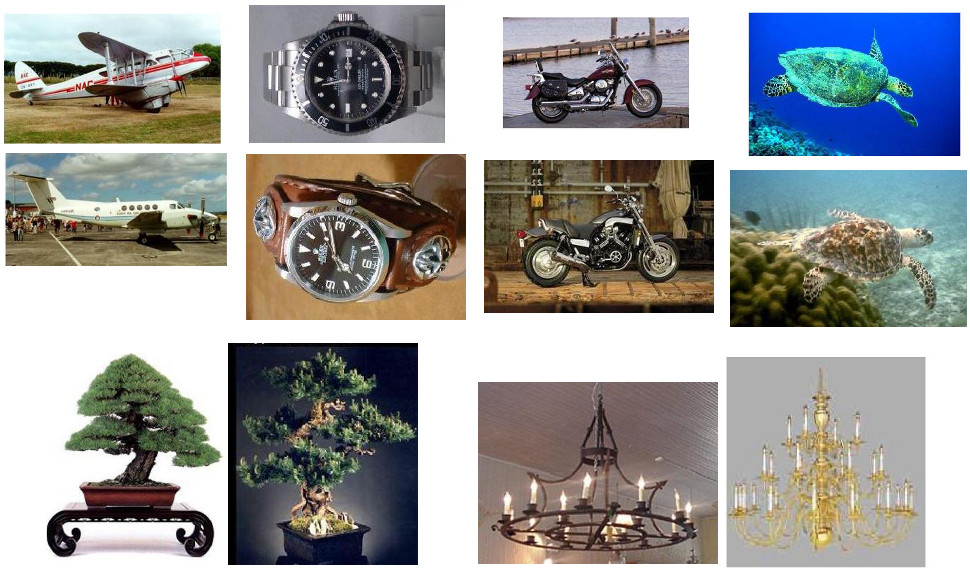
\includegraphics[width=.8\linewidth]{\detokenize{figuras/quantization/fig_Caltech101_dataset.jpg}}
        }
      \end{minipage}\par\medskip
      \centering
        \subfloat[Produce-1400]{
          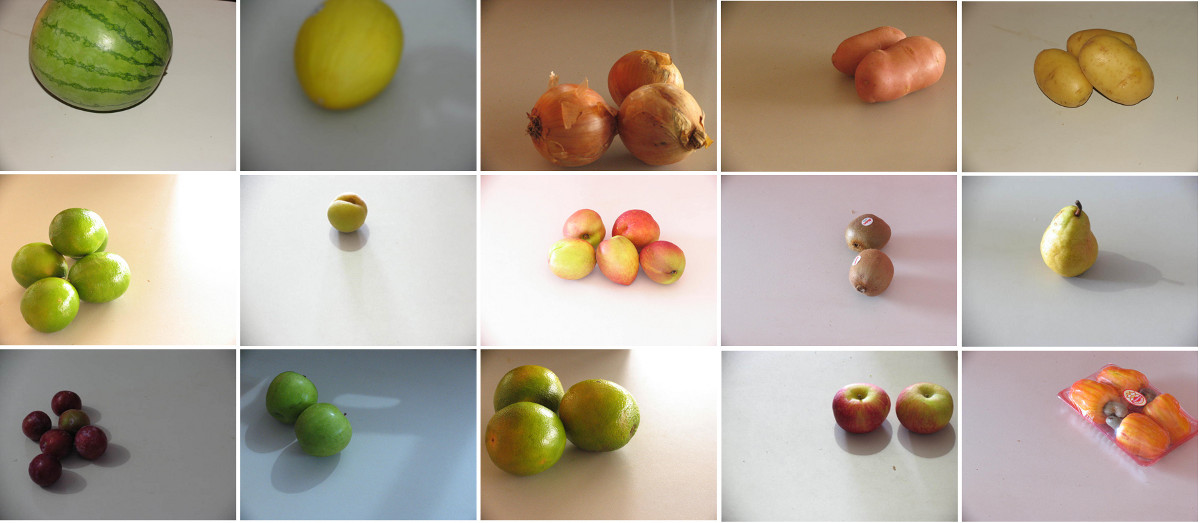
\includegraphics[width=.4\linewidth]{\detokenize{figuras/quantization/fig_Produce_dataset.jpg}}
        }
    \end{center}
    \caption{Bases de imagens utilizadas nos experimentos de quantização.}
  \end{figure}
\end{frame}
%-----------------------------------------------------------------------------
\begin{frame}{Experimentos --- Protocolo}
  \setstretch{1.2}
  \setlength\leftmargini{1em}
  \begin{block}{}
    \justifying
    \begin{enumerate}
      \item \textbf{Quantização}: \emph{Intensidade'}, \emph{Gleam}, \emph{Luminância'} e MSB.
      \item \textbf{Extração de características}
      \begin{itemize}
        \item \textit{Auto Color Correlogram} (ACC): quatro distâncias $d =$ 1, 3, 5 e 7;
        \item \textit{Border-Interior Classification} (BIC): vizinhança de quatro pixels;
        \item \textit{Color Coherence Vector} (CCV): $\mathit{threshold} = 25$;
        \item Haralick-6: pixel vizinho à direita.
      \end{itemize}
      \item \textbf{Redução da dimensionalidade}: \textit{Locality Preserving Projections} (LPP) com $d=$ 128, 64, 32 e 16 dimensões e $k=$ 10 vizinhos.
      \item \textbf{Classificação}: \textit{Support Vector Machines} (SVM) com \textit{grid search} no conjunto de treinamento.
    \end{enumerate}
  \end{block}
\end{frame}
%-----------------------------------------------------------------------------
% \begin{frame}{Experimentos --- Resultados}
%   \setstretch{1.2}
%   \setlength\leftmargini{1em}
%   \begin{block}{}
%     \justifying
%     \begin{enumerate}
%       \item
%     \end{enumerate}
%   \end{block}
% \end{frame}
%-----------------------------------------------------------------------------
\begin{frame}{Experimentos --- Resultados}
  \setstretch{1.2}
  \setlength\leftmargini{1em}
  \begin{figure}
    \begin{center}
      \centering
      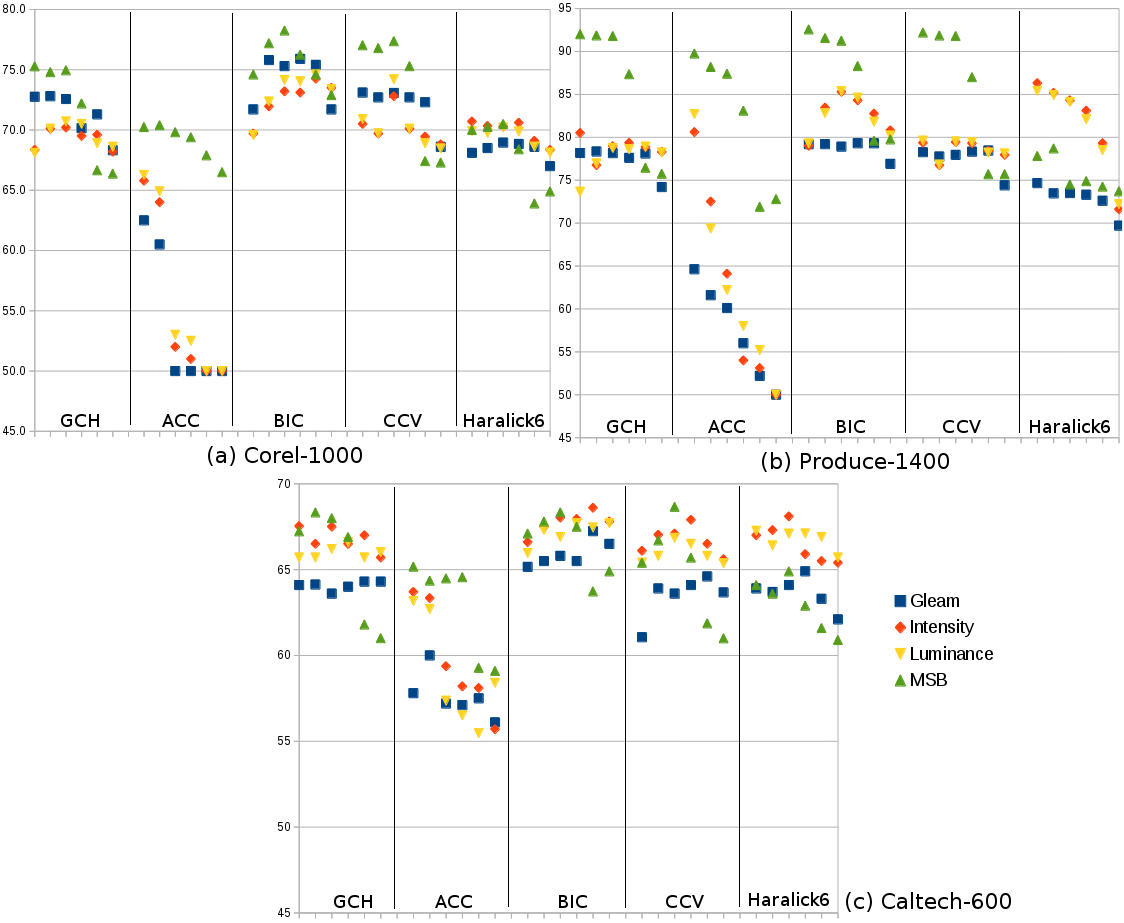
\includegraphics[width=.75\linewidth]{\detokenize{figuras/quantization/fig_results_individual.png}}
    \end{center}
    \caption{Acurácia média utilizando 256, 128, 64, 32, 16 e 8 cores.}
  \end{figure}
\end{frame}
%-----------------------------------------------------------------------------
\begin{frame}{Experimentos --- Resultados}
  \justifying
  \setstretch{1.2}
  \setlength\leftmargini{1em}
  \begin{figure}
    \begin{center}
      \centering
      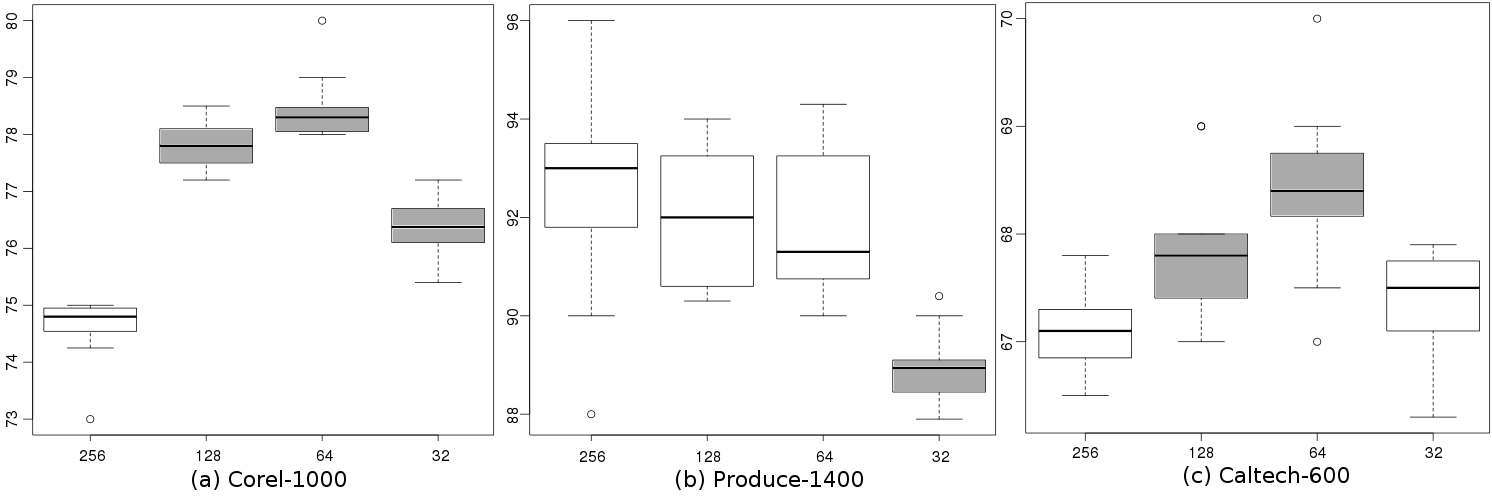
\includegraphics[width=\linewidth]{\detokenize{figuras/quantization/fig_results_individual_boxplotBIC.png}}
    \end{center}
    \caption{Acurácia média utilizando MSB e BIC ao variar o parâmetro de quantização. Os \textit{boxplots} em cinza correspondem às significâncias estatísticas com $\textit{p-value} < 0.01$ quando comparado à 256 cores. Converter para 64 cores prova ser boa escolha de processamento.}
  \end{figure}
\end{frame}
%-----------------------------------------------------------------------------
\begin{frame}{Experimentos --- Resultados}
  \setstretch{1.2}
  \setlength\leftmargini{1em}
  \begin{figure}
    \begin{center}
      \centering
      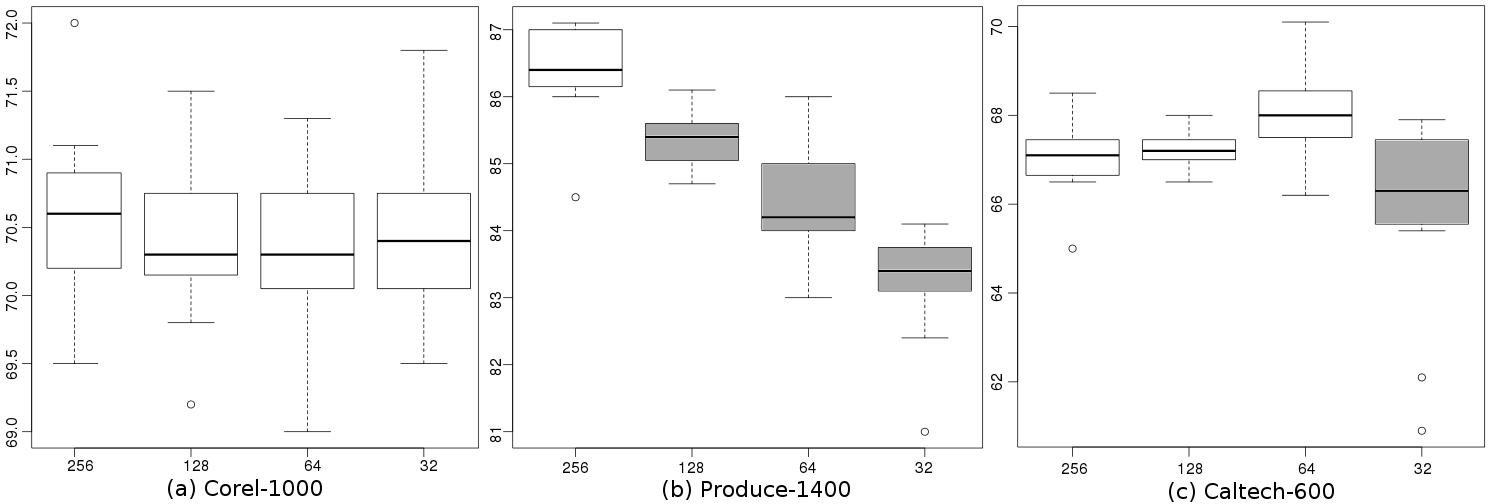
\includegraphics[width=\linewidth]{\detokenize{figuras/quantization/fig_results_individual_boxplotHaralick.png}}
    \end{center}
    \caption{Acurácia média utilizando \emph{Luminância'} e Haralick ao variar o parâmetro de quantização. Dependendo da base, a redução pode manter ou degradar a acurácia.}
  \end{figure}
\end{frame}
%-----------------------------------------------------------------------------
\begin{frame}{Experimentos --- Quantização versus LPP}
  \setstretch{1.2}
  \setlength\leftmargini{1em}
  \begin{itemize}
    \item Imagem convertida para escala de cinza com MSB em 256 cores;
    \item Extração de características com o método BIC;
    \item Vetor de entrada para LPP:
      \begin{itemize}
        \item Versões reduzidas de 256, 128 e 64 dimensões.
      \end{itemize}
    \item Comparação da acurácia dos vetores reduzidos pela quantização.
  \end{itemize}
\end{frame}
%-----------------------------------------------------------------------------
\begin{frame}{Experimentos --- Resultados da quantização versus LPP}
  \setstretch{1.2}
  \setlength\leftmargini{1em}
  \begin{figure}
    \begin{center}
      \centering
      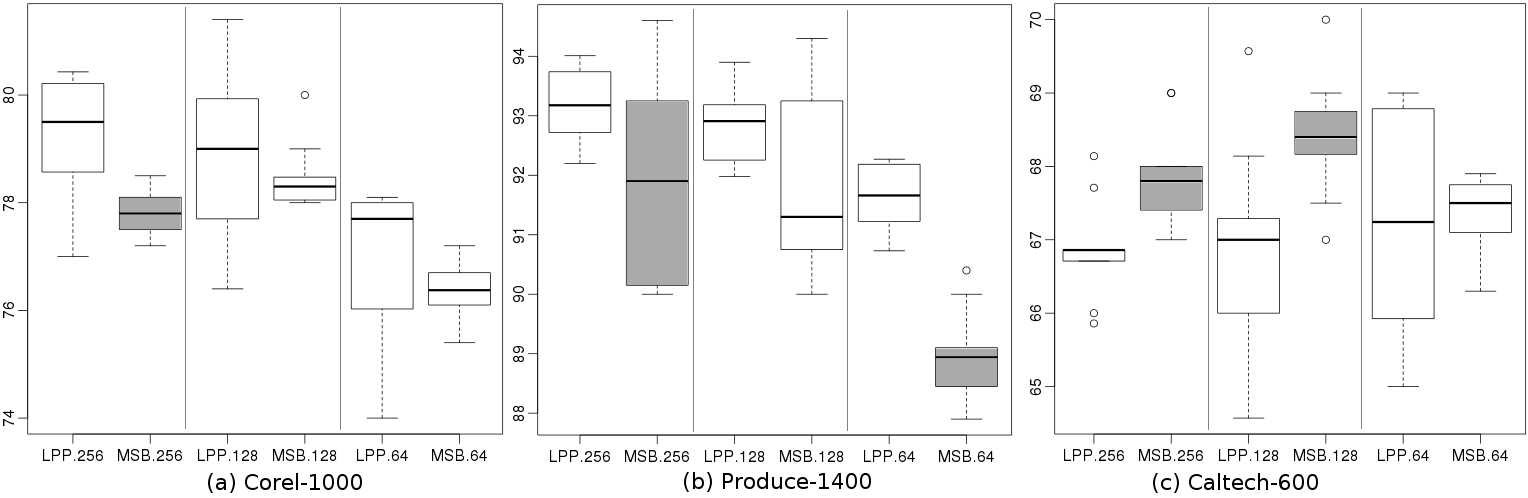
\includegraphics[width=\linewidth]{\detokenize{figuras/quantization/fig_results_individual_boxplotMSBLPP.png}}
    \end{center}
    \caption{Acurácia para os métodos MSB e LPP. A comparação foi realizada com a mesma dimensionalidade. Se utilizado um número de cores correto, é possível manter ou melhorar a acurácia.}
  \end{figure}
\end{frame}
%-----------------------------------------------------------------------------
\begin{frame}{Experimentos --- Concatenação}
  \setstretch{1.2}
  \setlength\leftmargini{1em}
  \begin{itemize}
    \item Número de dimensões de um único descritor pode ser baixo;
    \item Imagens convertidas em escala de cinza com 256 cores;
    \item Descritas por todos os métodos e suas características concatenadas em um vetor $D=2310$;
    \item Redução de dimensionalidade com LPP para $d=$ 1160, 582, 294 e 150. Mesmas dimensões de utilizar quantização como redução.
  \end{itemize}
\end{frame}
%-----------------------------------------------------------------------------
\begin{frame}{Experimentos --- Resultados da concatenação}
  \setstretch{1.2}
  \setlength\leftmargini{1em}
  \begin{figure}
    \begin{center}
      \centering
      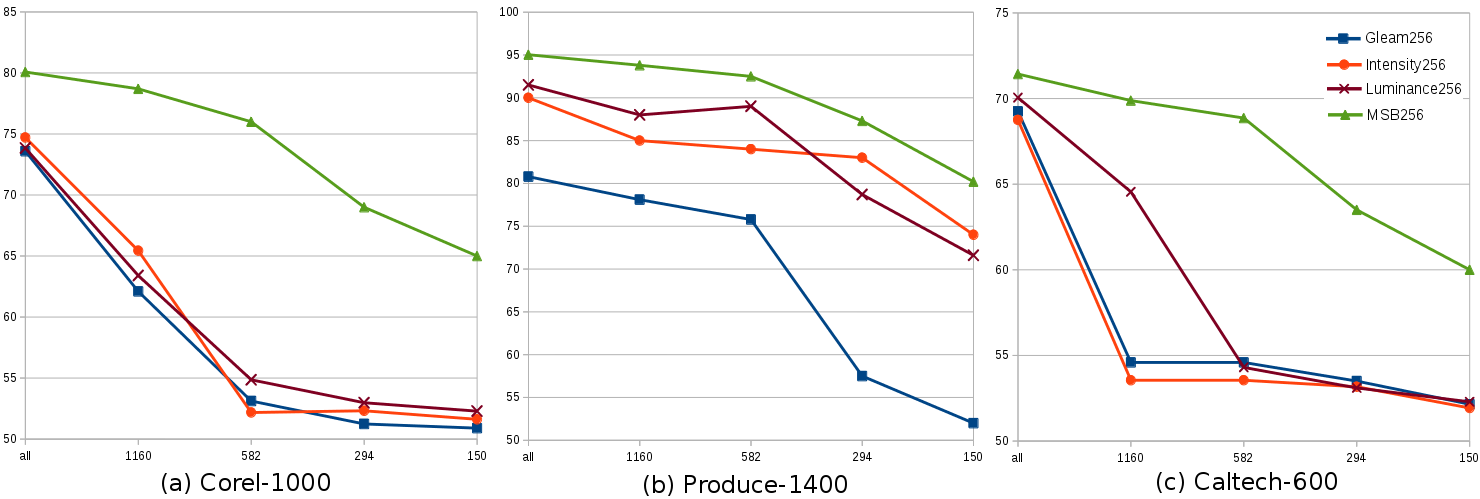
\includegraphics[width=\linewidth]{\detokenize{figuras/quantization/fig_results_full.png}}
    \end{center}
    \caption{Acurácia para \emph{Gleam}, \emph{Intensidade'}, \emph{Luminância'} e MSB. O vetor de características com $D=2310$ sofreu redução da dimensionalidade com o LPP para $d = 1160$, $582$, $294$ e $150$.}
  \end{figure}
\end{frame}
%-----------------------------------------------------------------------------
\begin{frame}{Experimentos --- Resultados da concatenação}
  \setstretch{1.2}
  \setlength\leftmargini{1em}
  \begin{figure}
    \begin{center}
      \centering
      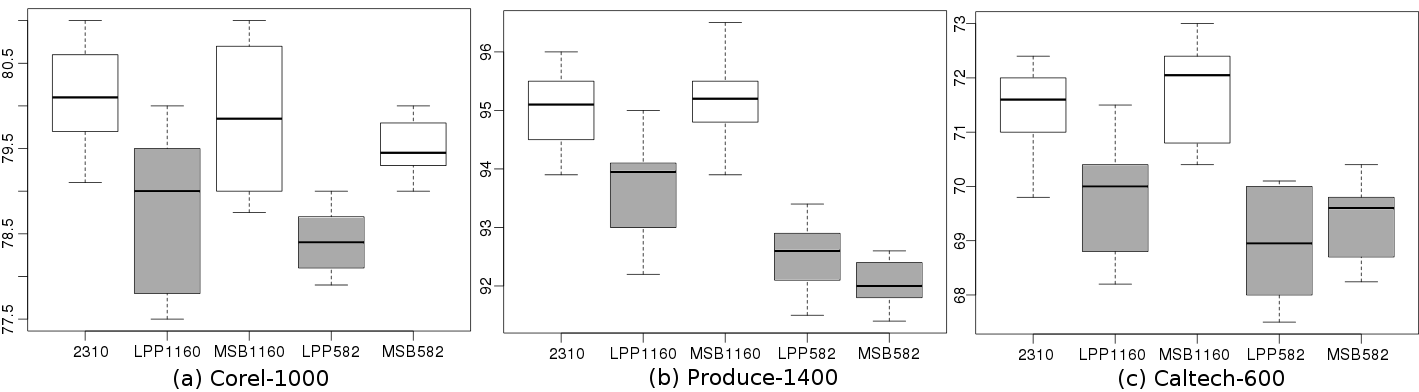
\includegraphics[width=\linewidth]{\detokenize{figuras/quantization/fig_results_full_boxplot.png}}
    \end{center}
    \caption{Comparação da redução de dimensionalidade obtida com LPP e MSB. Utilizar 128 ou 64 cores é indicado como uma boa escolha do parâmetro de quantização.}
  \end{figure}
\end{frame}
%-----------------------------------------------------------------------------
\begin{frame}{Experimentos --- Resultados da concatenação}
  \setstretch{1.2}
  \setlength\leftmargini{1em}
  \begin{figure}
    \begin{center}
      \centering
      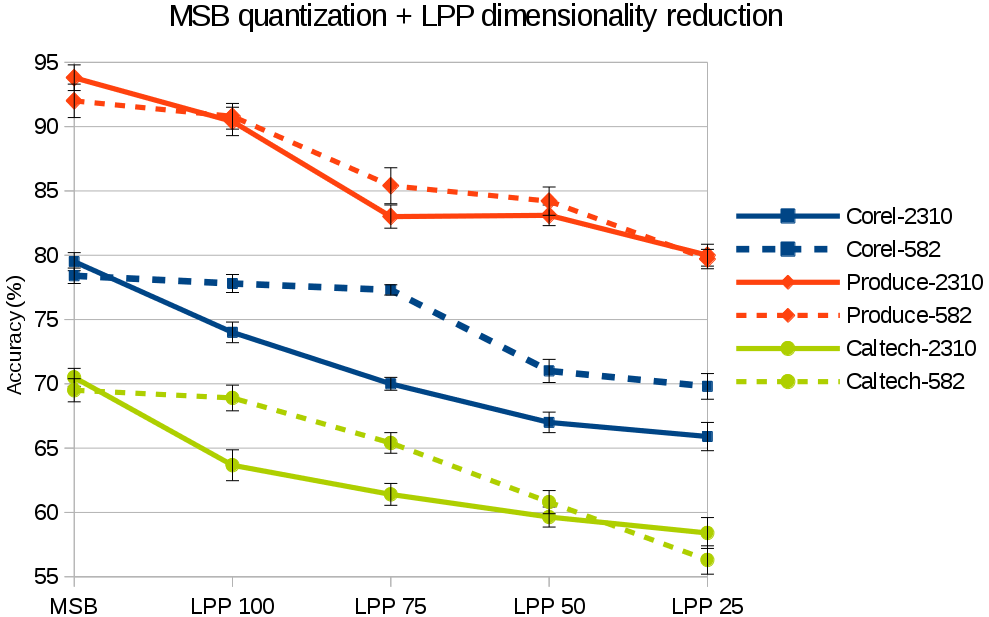
\includegraphics[width=0.6\linewidth]{\detokenize{figuras/quantization/fig_results_full_LPP}}
    \end{center}
    \caption{Projeção LPP sobre o espaço produzido pelo método MSB com 256 ($d = 2310$) e 64 cores ($d=582$). Em geral, as projeções com as imagens quantizadas em 64 cores foram melhores.}
  \end{figure}
\end{frame}
%-----------------------------------------------------------------------------
\begin{frame}{Experimentos --- Discussão}
  \setstretch{1.2}
  \setlength\leftmargini{1em}
  \begin{block}{}
    \justifying
    \begin{itemize}
      \item Aplicar a quantização na etapa de pré-processamento pode reduzir significativamente a dimensionalidade, enquanto melhora ou mantém a classificação do sistema;
      \item Inclusive quando comparado com métodos mais complexos para a redução da dimensionalidade;
      \item O vetor concatenado possui $9C + 6$ dimensões e o tempo de extração de todas as características é $f(N)=42N+6C^2$. Utilizar 64 cores ao invés de 256 para 100 imagens corresponde a uma redução de 74,6\% do número de instruções.
    \end{itemize}
  \end{block}
\end{frame}
%%%%%%%%%%%%%%%%%%%%%%%%%%%%%%%%%%%%%%%%%%%%%%%%%%%%%%%%%%%%%%%%%%%%%%%%%%%%%%%
\section{Geração de imagens artificiais}
\subsection{Contextualização}
\begin{frame}{Desbalanceamento de classes}
  \setstretch{1.2}
  \setlength\leftmargini{1em}
  \justifying
  \setstretch{1.2}
  \begin{itemize}
    \item Número desbalanceado de exemplos: majoritárias x minoritárias;
    \item Abordagens:
    \begin{itemize}
      \item \emph{Pré-processamento ao reamostrar os dados:}
      \begin{itemize}
        \item Aumentar a minoritária (Em geral, melhores resultados);
        \item Diminuir a majoritária.
      \end{itemize}
      \item \emph{Modificar métodos de aprendizagem:} adicionar funções de custo na classificação;
    \end{itemize}
  \end{itemize}
\end{frame}
%-----------------------------------------------------------------------------
\begin{frame}{Desbalanceamento de classes --- Subamostragem}
  \setstretch{1.2}
  \setlength\leftmargini{1em}
  \justifying
  \begin{itemize}
    \item Diminuir o número de elementos do conjunto;
    \item Eliminar elementos distantes da fronteira de decisão (menos relevantes);
    \item Normalmente apresentam resultados piores;
    \item Pode remover informações essenciais dos dados originais;
    \item Não há melhor para todos os cenários.
  \end{itemize}
\end{frame}
%-----------------------------------------------------------------------------
\begin{frame}{Desbalanceamento de classes --- Sobreamostragem}
  \setstretch{1.2}
  \setlength\leftmargini{1em}
  \justifying
  \begin{itemize}
    \item Aumentar o número de elementos;
    \begin{block}{SMOTE (Chawla et al., 2002)}
      \setlength\leftmargini{1em}
      \begin{itemize}
        \item Multiplica a diferença entre o vetor de características de um elemento e do seu vizinho mais próximo por um número $0 \leq x \leq 1$;
        \item Adiciona ao vetor original, criando um novo elemento entre os dois vetores originais;
        \item Aprendido como exemplo da classe minoritária;
      \end{itemize}
    \end{block}
  \end{itemize}
\end{frame}
%-----------------------------------------------------------------------------
% \begin{frame}{Desbalanceamento de classes --- Sobreamostragem}
%   \setstretch{1.2}
%   \setlength\leftmargini{1em}
%   \footnotesize{
%   \justifying
%   \begin{block}{}
%     \begin{algorithm}[H]
%       \caption{SMOTE: método para rebalancear classes}
%       \SetAlgoLined
%       \Entrada{Imagem colorida $I$ em formato RGB}
%       \Saida{Exemplos sintéticos $S$}
%       $N \gets \textit{vizinhos(classe minoritária)}$\;
%       \ParaCada{exemplo da classe minoritária}{
%       $nn \gets \textit{vizinho aleatório de N}$\;
%       $\textit{novo\_elemento} \gets \emptyset $\;
%
%       \ParaCada{\textit{característica} $(x,y)$ do exemplo}{
%       $\textit{diferença} \gets nn(x,y) - exemplo(x,y)$\;
%       $\textit{gap} \gets \textit{número aleatório entre 0 e 1}$\;
%       $\textit{novo\_elemento}(x,y) \gets exemplo(x,y) + gap*\textit{diferença}$\;
%       }
%       $S \gets S \cup \textit{novo\_elemento}$\;
%       }
%     \end{algorithm}
%   \end{block}
%   }
% \end{frame}
%-----------------------------------------------------------------------------
\begin{frame}{Desbalanceamento de classes --- SMOTE}
  \setstretch{1.2}
  \setlength\leftmargini{1em}
  \justifying
  \begin{figure}[hbpt]
    \begin{center}
      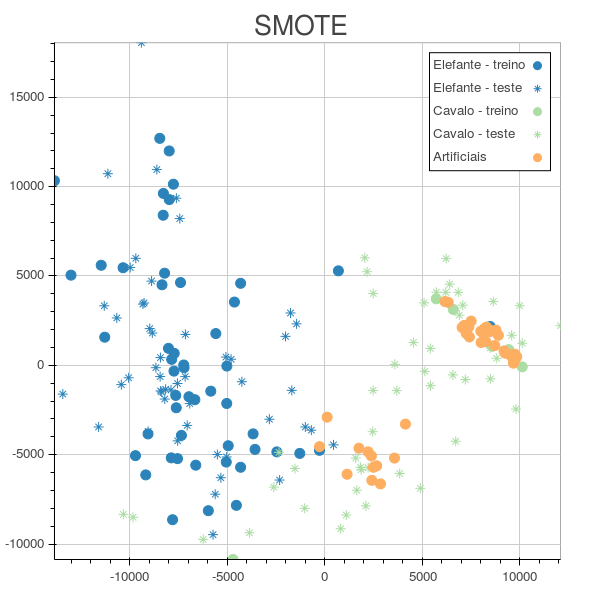
\includegraphics[width=.5\linewidth]{{figuras/smote}}
    \end{center}
    \caption{SMOTE}
  \end{figure}
  \justifying
  \begin{itemize}
    \item Força uma região de decisão maior e mais geral;
    \item Rebalancear ao gerar novos elementos, ao invés de replicá-los;
    % \item Sobre os vetores de características previamente extraídos;
    \item \textbf{Diferentes estratégias para criar exemplos sintéticos podem melhorar a performance da classificação};
    \item Utilizado para comparação.
  \end{itemize}
\end{frame}
%%%%%%%%%%%%%%%%%%%%%%%%%%%%%%%%%%%%%%%%%%%%%%%%%%%%%%%%%%%%%%%%%%%%%%%%%%%%%%%
\subsection{Método}
\begin{frame}{Geração de imagens artificiais}
  \setstretch{1.2}
  \setlength\leftmargini{1em}
  \begin{block}{}
    \justifying
    \begin{itemize}
      \item Compensar a baixa disponibilidade de exemplos de uma determinada classe;
      \item Permitir a extração de informações antes não disponíveis nas imagens originais por meio da combinação ou perturbação das imagens de entrada.
    \end{itemize}
  \end{block}
\end{frame}
%-----------------------------------------------------------------------------
\begin{frame}{Geração de imagens artificiais}
  \setstretch{1.2}
  \setlength\leftmargini{1em}
  \begin{figure}
    \begin{center}
      \includegraphics[width=0.6\linewidth]{\detokenize {figuras/rebalance.pdf}}
    \end{center}
    \caption{Geração de imagens artificiais da classe minoritária para rebalancear a base de imagens.}
  \end{figure}
\end{frame}
%-----------------------------------------------------------------------------
% \begin{frame}{Geração de imagens artificiais --- Métodos}
%   \setstretch{1.2}
%   \setlength\leftmargini{1em}
%   \begin{block}{}
%     \justifying
%     \begin{itemize}
%       \item Borramento;
%       \item Aguçamento;
%       \item Composição;
%       \item Mistura ponderada;
%       \item Mistura limiarizada;
%       \item Mistura saliente;
%       \item SMOTE visual;
%       \item Adição de ruído.
%     \end{itemize}
%   \end{block}
% \end{frame}
%-----------------------------------------------------------------------------
\begin{frame}{Geração de imagens artificiais --- Borramento}
  \setstretch{1.2}
  \setlength\leftmargini{1em}
  \begin{figure}
    \begin{center}
      \subfloat[Original]{
      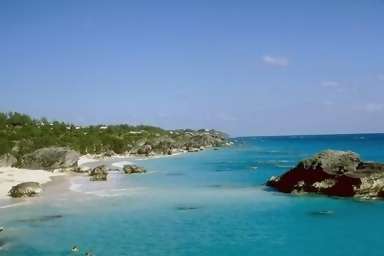
\includegraphics[width=.48\linewidth]{\detokenize{figuras/artificial-generation/methods/blur-a.png}}
      }
      \subfloat[Imagem artificial]{
      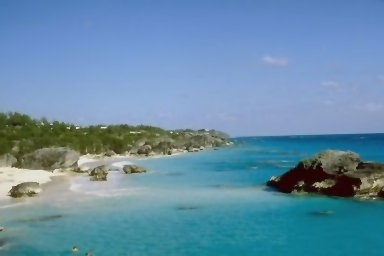
\includegraphics[width=.48\linewidth]{\detokenize{figuras/artificial-generation/methods/blur-b.png}}
      }
    \end{center}
    \caption{Filtro bilateral. A imagem (b) possui detalhes borrados, porém preservando as bordas.}
  \end{figure}
\end{frame}
%-----------------------------------------------------------------------------
\begin{frame}{Geração de imagens artificiais --- Aguçamento}
  \setstretch{1.2}
  \setlength\leftmargini{1em}
  \begin{figure}
    \begin{center}
      \subfloat[Original]{
      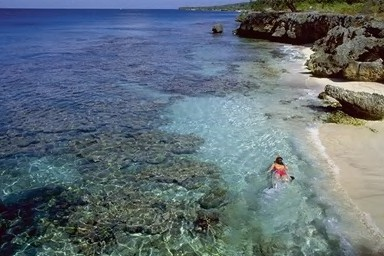
\includegraphics[width=.48\linewidth]{\detokenize{figuras/artificial-generation/methods/unsharp-a.png}}
      }
      \subfloat[Imagem artificial]{
      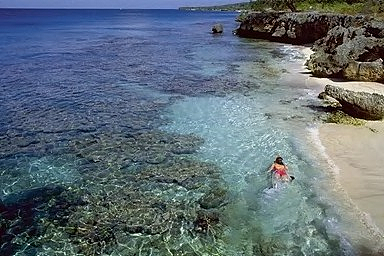
\includegraphics[width=.48\linewidth]{\detokenize{figuras/artificial-generation/methods/unsharp-b.png}}
      }
    \end{center}
    \caption{\textit{Unsharp mask}. A imagem resultante (b) apresenta saliência nas transições de intensidade.}
  \end{figure}
\end{frame}
%-----------------------------------------------------------------------------
\begin{frame}{Geração de imagens artificiais --- Adição de ruído}
  \setstretch{1.2}
  \setlength\leftmargini{1em}
  \begin{figure}
    \begin{center}
      \subfloat[Original]{
      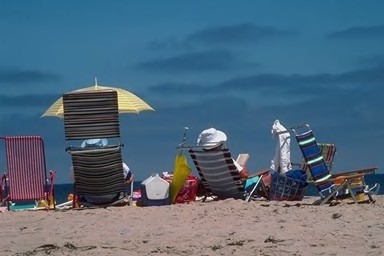
\includegraphics[width=.48\linewidth]{\detokenize{figuras/artificial-generation/methods/noise-a.png}}
      }
      \subfloat[Imagem artificial]{
      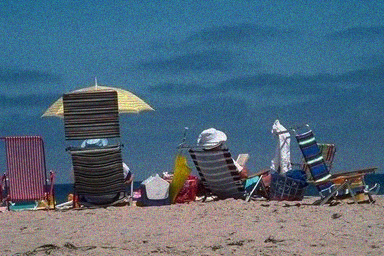
\includegraphics[width=.48\linewidth]{\detokenize{figuras/artificial-generation/methods/noise-b.png}}
      }
    \end{center}
    \caption{Ruído de Poisson. Regiões claras de (b) apresentam mais ruído que as regiões escuras.}
  \end{figure}
\end{frame}
%-----------------------------------------------------------------------------
\begin{frame}{Geração de imagens artificiais --- SMOTE visual}
  \setstretch{1.2}
  \setlength\leftmargini{1em}
  \begin{figure}
    \begin{center}
      \subfloat[Original]{
      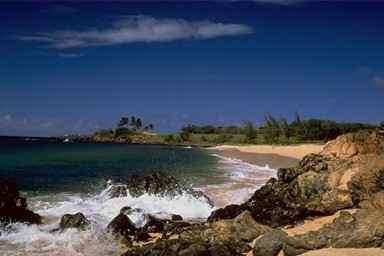
\includegraphics[height=2.8cm,keepaspectratio]{\detokenize{figuras/artificial-generation/methods/smote-a.png}}
      }
      \subfloat[Original]{
      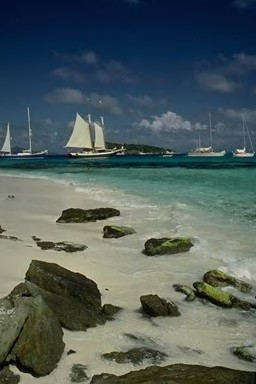
\includegraphics[height=2.8cm,keepaspectratio]{\detokenize{figuras/artificial-generation/methods/smote-b.png}}
      }
      \subfloat[Imagem artificial]{
      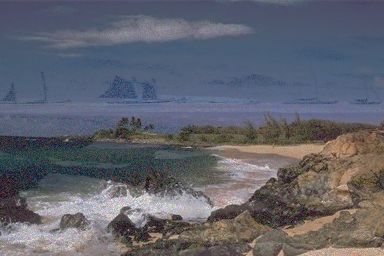
\includegraphics[height=2.8cm,keepaspectratio]{\detokenize{figuras/artificial-generation/methods/smote-c.png}}
      }
    \end{center}
    \caption{Smote ao nível de pixels. É possível notar a sobreposição de uma ``sombra'' da Figura (b) em (a).}
  \end{figure}
\end{frame}
%-----------------------------------------------------------------------------
\begin{frame}{Geração de imagens artificiais --- Mistura ponderada}
  \setstretch{1.2}
  \setlength\leftmargini{1em}
  \begin{figure}
    \begin{center}
      \subfloat[Original]{
      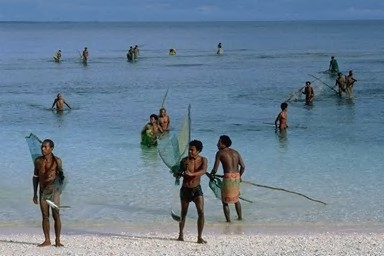
\includegraphics[width=.32\linewidth]{\detokenize{figuras/artificial-generation/methods/blend-a.png}}
      }
      \subfloat[Original]{
      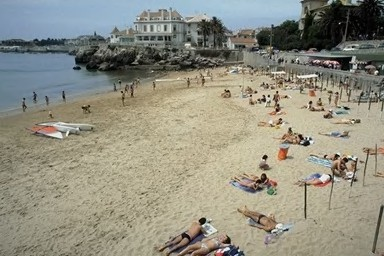
\includegraphics[width=.32\linewidth]{\detokenize{figuras/artificial-generation/methods/blend-b.png}}
      }
      \subfloat[Imagem artificial]{
      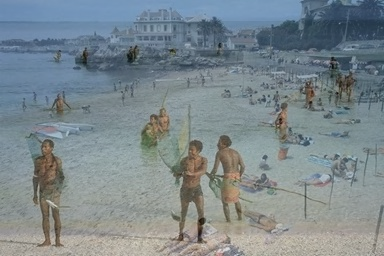
\includegraphics[width=.32\linewidth]{\detokenize{figuras/artificial-generation/methods/blend-c.png}}
      }
    \end{center}
    \caption{Soma ponderada de duas imagens. A imagem (c) representa a mistura de (a) e (b).}
    \label{fig:gen:blend}
  \end{figure}
\end{frame}
%-----------------------------------------------------------------------------
\begin{frame}{Geração de imagens artificiais --- Mistura limiarizada}
  \setstretch{1.2}
  \setlength\leftmargini{1em}
  \begin{figure}
    \begin{center}
      \subfloat[Original]{
      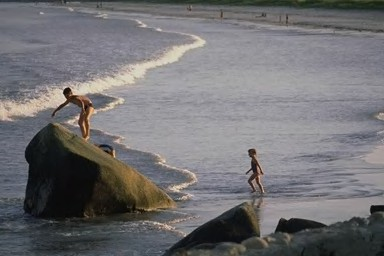
\includegraphics[width=.32\linewidth]{\detokenize{figuras/artificial-generation/methods/threshold-a.png}}
      }
      \subfloat[Original]{
      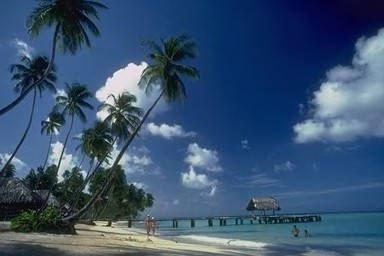
\includegraphics[width=.32\linewidth]{\detokenize{figuras/artificial-generation/methods/threshold-b.png}}
      }
      \subfloat[Imagem artificial]{
      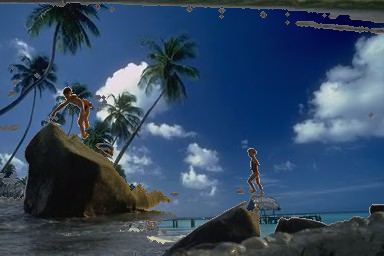
\includegraphics[width=.32\linewidth]{\detokenize{figuras/artificial-generation/methods/threshold-c.png}}
      }
    \end{center}
    \caption{Mistura de \textit{thresholds}. A imagem resultante (c) é uma composição do \textit{foreground} da primeira imagem sobre a segunda.}
  \end{figure}
\end{frame}
%-----------------------------------------------------------------------------
\begin{frame}{Geração de imagens artificiais --- Mistura saliente}
  \setstretch{1.2}
  \setlength\leftmargini{1em}
  \begin{figure}
    \begin{center}
      \subfloat[Original]{
      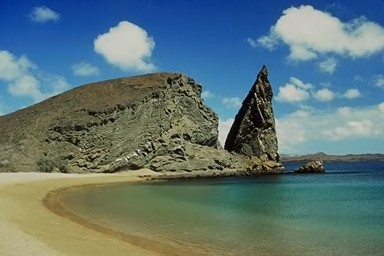
\includegraphics[width=.32\linewidth]{\detokenize{figuras/artificial-generation/methods/saliency-a.png}}
      }
      \subfloat[Original]{
      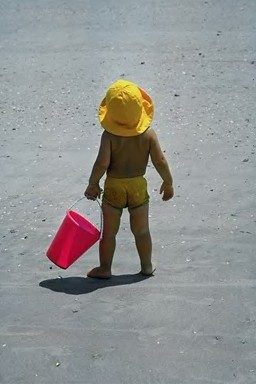
\includegraphics[width=.32\linewidth]{\detokenize{figuras/artificial-generation/methods/saliency-b.png}}
      }
      \subfloat[Imagem artificial]{
      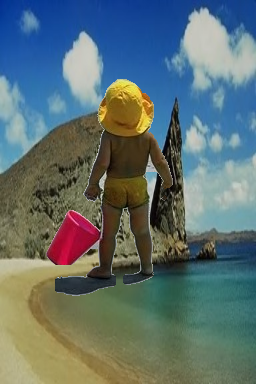
\includegraphics[width=.32\linewidth]{\detokenize{figuras/artificial-generation/methods/saliency-c.png}}
      }
    \end{center}
    \caption{Combinação de saliência. A imagem resultante (c) apresenta a região saliente de (b) sobreposta em (a).}
  \end{figure}
\end{frame}
%-----------------------------------------------------------------------------
\begin{frame}{Geração de imagens artificiais --- Composição}
  \setstretch{1.2}
  \setlength\leftmargini{1em}
  \begin{figure}
    \begin{center}
      \centering
      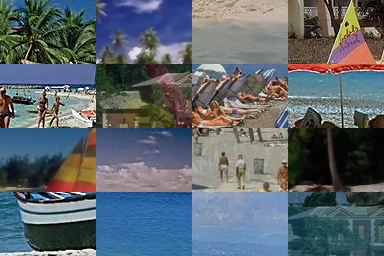
\includegraphics[width=0.6\linewidth]{\detokenize{figuras/artificial-generation/methods/composition.png}}
    \end{center}
    \caption{Várias imagens, dispostas em um mosaico, formam a imagem resultante. Cada célula do mosaico sofre uma operação, sorteada no momento da geração da imagem.}
  \end{figure}
\end{frame}
%-----------------------------------------------------------------------------
\subsection{Experimentos}
\begin{frame}{Experimentos}
  \setstretch{1.2}
  \setlength\leftmargini{1em}
  \begin{block}{}
    \justifying
      Comparar a classificação:
      \begin{itemize}
        \item Base original;
        \item Geração de imagens artificiais com os métodos anteriores;
        \item Técnica de sobreamostragem SMOTE.
      \end{itemize}
  \end{block}
\end{frame}
%-----------------------------------------------------------------------------
\begin{frame}
  \setstretch{1.2}
  \setlength\leftmargini{1em}
  \begin{figure}
    \centering
    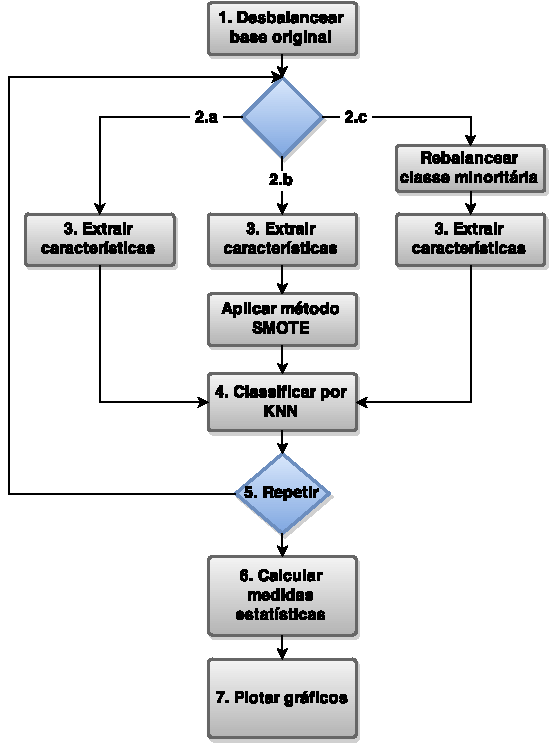
\includegraphics[scale=.58]{\detokenize{figuras/flow_main.pdf}}
    \caption{Fluxo de operações para obtenção dos resultados do rebalanceamento de classes.}
% O mesmo protocolo de conversão para escala de cinza, extração de características e classificação foi seguido para três sub-experimentos: base desbalanceada; base rebalanceada com interpolação dos vetores de características (método SMOTE); e base rebalanceada com a geração artificial de imagens.}
  \end{figure}
\end{frame}
% %-----------------------------------------------------------------------------
% \begin{frame}{Avaliação da Classificação}
% % \setstretch{1.2}
% \setlength\leftmargini{1em}
% \begin{block}{Medida F1}
% \justifying
% Problema da acurácia: minoritária sem resultados corretos. \\
% % Performance da classificação em cenários desbalanceados.
% \begin{itemize}
%
% \item Precisão (exatidão): dos exemplos classificados como positivos, quantos realmente são.
% \vspace{-1.5em}
% \begin{equation*}
%   P = \frac{VP}{VP + FP}
% \end{equation*}
% \item Revocação (completude): exemplos positivos corretamente classificados como tal.
% \begin{equation*}
%   R = \frac{VP}{VP + FN}
% \end{equation*}
%
% \pause
% \begin{equation*}
%   F1 = 2 \frac{P \cdot R}{P+R}
% \end{equation*}
% \end{itemize}
% \end{block}
% \end{frame}
%%%%%%%%%%%%%%%%%%%%%%%%%%%%%%%%%%%%%%%%%%%%%%%%%%%%%%%%%%%%%%%%%%%%%%%%%%%%%%%
\begin{frame}{Experimento --- Visualização}
  \setstretch{1.2}
  \setlength\leftmargini{1em}
  \begin{itemize}
  \item Visualização do espaço obtido após a geração de imagens;
  \item Verificar a definição da classe minoritária em relação ao espaço original;
  \item Analisar qual método mais se assemelha à distribuição original dos dados.
  \end{itemize}
\end{frame}
%-----------------------------------------------------------------------------
\begin{frame}[allowframebreaks]{Protocolo --- Visualização}
\justify
  \setstretch{1.5}
  \setlength\leftmargini{1em}
  \begin{enumerate}
    \item \textbf{Imagens originais}: \emph{Horse} e \emph{Elephant} com 100 imagens cada;
    \begin{figure}
      \begin{center}
        \subfloat[Elephant]{
        \includegraphics[width=0.4\linewidth]{\detokenize{figuras/corel_original4.jpg}}
        }
        \subfloat[Horse]{
        \includegraphics[width=0.4\linewidth]{\detokenize{figuras/cavalo-original2.png}}
        }
        \caption{Originalmente da base de imagens Corel-1000, a principal característica dessas imagens é a diferença de cores, contendo pequeno grau de sobreposição.}
      \end{center}
    \end{figure}
%%%%%%%%%%%%%%%%%%
    \item \textbf{Desbalanceamento}: cada classe foi dividida em 50\% para treino e 50\% para teste, de maneira aleatória. Após, a classe \emph{Horse} sofreu remoção de 50\% do seu conjunto de treino;
    \framebreak
%%%%%%%%%%%%%%%%%%
    \item \textbf{Método para geração de imagens}: \emph{mistura ponderada};

  \begin{figure}
    \begin{center}
      \subfloat[Original]{
      \includegraphics[width=.32\linewidth]{\detokenize{figuras/cavalo-original.png}}
      }
      \subfloat[Original]{
      \includegraphics[width=.32\linewidth]{\detokenize{figuras/cavalo-original2.png}}
      }
      \subfloat[Imagem artificial]{
      \includegraphics[width=.32\linewidth]{\detokenize{figuras/cavalo-blend.png}}
      }
      \caption{Mistura ponderada. A imagem resultante (c) é composta pela mistura de (a) e (b).}
    \end{center}
  \end{figure}

    \item \textbf{Conversão em escala de cinza}: \emph{Intensidade'};

    \item \textbf{Extração de características}: BIC;
%%%%%%%%%%%%%%%%%%
    \item \textbf{Classificação}: KNN com $K=1$;

    \item \textbf{Projeção multidimensional para visualização}: projetados os dois componentes principais encontrados ao aplicar PCA nos vetores de características.
  \end{enumerate}
\end{frame}
%-----------------------------------------------------------------------------
\begin{frame}{Experimento --- Visualização}
  \setstretch{1.2}
  \setlength\leftmargini{1em}
  \begin{figure}
    \begin{center}
      \subfloat[Original]{
      \includegraphics[width=.45\linewidth]{\detokenize{figuras/visualizacao/original.png}}
      }
      \subfloat[Desbalanceado]{
      \includegraphics[width=.45\linewidth]{\detokenize{figuras/visualizacao/desbalanceado-fixed.png}}
      }
    \end{center}
    \caption{Projeção dos dois componentes principais obtidos com o PCA. À direita, as mesmas classes após a remoção de 50\% do treino da classe \emph{Horse}.}
  \end{figure}
\end{frame}
%-----------------------------------------------------------------------------
\begin{frame}{Experimento --- Visualização}
  \setstretch{1.2}
  \setlength\leftmargini{1em}
  \begin{figure}
    \begin{center}
      \subfloat[SMOTE]{
      \includegraphics[width=.45\linewidth]{\detokenize{figuras/visualizacao/smote-treino-fixed.png}}
      }
      \subfloat[Geração de imagens artificiais]{
      \includegraphics[width=.45\linewidth]{\detokenize{figuras/visualizacao/geracao-treino-fixed.png}}
      }
    \end{center}
    \caption{Novos exemplos de treinamento da geração com SMOTE e no campo visual com o método \emph{mistura} (em laranja). Ganho de mais de 10\% de acurácia.}
  \end{figure}
\end{frame}
%-----------------------------------------------------------------------------
\begin{frame}{Experimento --- Visualização}
  \setstretch{1.2}
  \setlength\leftmargini{1em}
  \begin{figure}
    \begin{center}
      \subfloat[Smote]{
      \includegraphics[width=.45\linewidth]{\detokenize{figuras/visualizacao/smote-teste-fixed.png}}
      }
      \subfloat[Geração de imagens]{
      \includegraphics[width=.45\linewidth]{\detokenize{figuras/visualizacao/geracao-teste-fixed.png}}
      }
    \end{center}
    \caption{A cor da borda dos marcadores representa a classe predita pelo classificador K-NN com $K = 1$ após o treinamento realizado com as bases rebalanceadas.}
  \end{figure}
\end{frame}
%-----------------------------------------------------------------------------
\begin{frame}{Experimento --- Visualização}
  \setstretch{1.2}
  \setlength\leftmargini{1em}
  \begin{itemize}
    \item A geração de imagens melhorou a definição da classe minoritária;
    \item Se assemelhou à distribuição dos dados originais;
    \item Ao interpolar os vetores originais o SMOTE pode criar exemplos em regiões que pertencem a outra classe;
    \item Além disso, não extrapolou a sua região.
  \end{itemize}
\end{frame}
%-----------------------------------------------------------------------------
\begin{frame}{Experimento --- Visualização}
  \setstretch{1.2}
  \setlength\leftmargini{1em}
  \begin{figure}
    \begin{center}
      \subfloat[Desbalanceado]{
      \includegraphics[width=.32\linewidth]{\detokenize{figuras/visualizacao/desbalanceado-teste-region.png}}
      }
      \subfloat[Smote]{
      \includegraphics[width=.32\linewidth]{\detokenize{figuras/visualizacao/smote-teste-region.png}}
      }
      \subfloat[Geração de imagens]{
      \includegraphics[width=.32\linewidth]{\detokenize{figuras/visualizacao/geracao-teste-region.png}}
      }
    \end{center}
    \caption{Região de decisão com 1-NN. A classe minoritária apresenta-se melhor representada e o SMOTE ocasionou uma certa invasão do espaço de características da classe majoritária.}
  \end{figure}
\end{frame}
%-----------------------------------------------------------------------------
\begin{frame}{Experimento --- Visualização}
  \setstretch{1.2}
  \setlength\leftmargini{1em}
  \begin{figure}
    \begin{center}
      \subfloat[Desbalanceado]{
      \includegraphics[width=.32\linewidth]{\detokenize{figuras/visualizacao/desbalanceado-treino.png}}
      }
      \subfloat[Smote]{
      \includegraphics[width=.32\linewidth]{\detokenize{figuras/visualizacao/smote-treino.png}}
      }
      \subfloat[Geração de imagens]{
      \includegraphics[width=.32\linewidth]{\detokenize{figuras/visualizacao/geracao-treino.png}}
      }
    \end{center}
    \caption{Melhores subespaços encontrados (componentes recalculadas). A geração de imagens artificiais proporciona a criação de um subespaço que melhor discretiza as classe.}
  \end{figure}
\end{frame}
%-----------------------------------------------------------------------------
\begin{frame}{Experimento --- Visualização}
  \setstretch{1.2}
  \setlength\leftmargini{1em}
  \begin{figure}
    \begin{center}
      \includegraphics[width=.58\linewidth]{\detokenize{figuras/visualizacao/vis-images.png}}
    \end{center}
    \caption{Impacto do método de extração de características BIC na separação entre classes.}
  \end{figure}
\end{frame}
%-----------------------------------------------------------------------------
\begin{frame}{Experimentos --- Validação}
  \setstretch{1.2}
  \setlength\leftmargini{1em}
  \begin{figure}
    \centering
    \includegraphics[scale=.12]{\detokenize{figuras/folds_chart.png}}
    \caption{Validação \textit{k-fold} com o objetivo de prover mais robustez ao sistema.}
% Primeiramente as imagens são separadas de forma aleatória em $k = 5$ \textit{folds} em cada classe. Em seguida, as duas classes compõem 40 configurações, consistindo em todas as possibilidades de: um fold para teste e os outros como treino para a classe que permanecerá balanceada; e um de teste e apenas um de treino para a classe que os métodos de processamento irão rebalancear. Tal validação é repetida para todas as classes, ou seja, cada classe tem a possibilidade de ser a minoritária.}
  \end{figure}
\end{frame}
%-----------------------------------------------------------------------------
\begin{frame}{Experimento}
  \setstretch{1.2}
  \setlength\leftmargini{1em}
  \begin{figure}
    \begin{center}
      \includegraphics[width=.8\linewidth]{\detokenize{figuras/artificial-generation/1/ACC_Gleam_elefante-cavalo.png}}
    \end{center}
    \caption{Boxplot para os métodos \emph{Gleam} e ACC, combinação com melhor F1-Score para \textit{Horse} e \textit{Elephant}.}
  \end{figure}
\end{frame}
%-----------------------------------------------------------------------------
\begin{frame}{Experimento}
  % \setstretch{1.2}
  \setlength\leftmargini{1em}
  \begin{table}
    \begin{center}
      \caption{A geração com \textit{Composição 4} obteve maior valor de \textit{F1-Score}. Difere do resultado utilizando BIC e Intensidade'.}
      \tiny{
        \begin{tabular}{|l|c|c|}
          \hline
          \textbf{\emph{Gleam} \& ACC} & \textbf{Média}     & \textbf{Desvio Padrão} \\ \hline
          Todos                 & 91.090913          & 4.559066               \\ \hline
          Aguçamento            & 91.002678          & 4.907016               \\ \hline
          Borramento            & 89.394500          & 5.103498               \\ \hline
          Composição 16         & 90.934305          & 4.399334               \\ \hline
          Composição 4          & \textbf{91.773528} & 4.909852               \\ \hline
          Limiares              & 90.893133          & 5.285833               \\ \hline
          Mistura               & 90.177055          & 4.409787               \\ \hline
          Ruído                 & 89.337770          & 5.169757               \\ \hline
          SMOTE Visual          & 88.616535          & 5.567976               \\ \hline
          Saliência             & 91.282655          & 4.230281               \\ \hline
          SMOTE                 & 90.173808          & 4.566863               \\ \hline
          Desbalanceado         & 88.258567          & 5.538461               \\ \hline
        \end{tabular}
      }
    \end{center}
  \end{table}
\end{frame}
%-----------------------------------------------------------------------------
\begin{frame}{Experimento}
  \setstretch{1.2}
  \setlength\leftmargini{1em}
  \begin{figure}
    \begin{center}
      \subfloat[Imagem gerada]{
      \includegraphics[width=.6\linewidth]{\detokenize{figuras/artificial-generation/1/resultado-composicao.png}}
      }
    \end{center}
    \caption{A imagem gerada apresenta uma \emph{composição} de quatro imagens da classe \textit{Elephant}.}
  \end{figure}
\end{frame}
%-----------------------------------------------------------------------------
\begin{frame}{Teste \textit{post-hoc} HSD de Tukey}
  \setstretch{1.2}
  \setlength\leftmargini{1em}
  \begin{itemize}
    \item Não há diferença estatística relevante entre a base desbalanceada e o SMOTE ($\textit{p-value}=0.2073$);
    \item Significância entre o desbalanceamento e a geração de imagens ($\textit{p-value}=0.0062$);
    \item O melhor método para rebalancear essas classes é a geração de imagens utilizando o método de composição de quatro imagens.
  \end{itemize}
\end{frame}
%-----------------------------------------------------------------------------
\begin{frame}{\textit{Ranking} dos métodos de rebalanceamento}
  \setstretch{1.2}
  \setlength\leftmargini{1em}
  \begin{table}
    \centering
    \caption{Resultados acumulados de todos os experimentos. Diferenças não significativas de F1-Score possuem o mesmo peso que as significantes.}
    \tiny{
    \begin{tabular}{|l|l|l|}
      \hline
      \multicolumn{1}{|c|}{\textbf{Cenários de duas classes}} & \multicolumn{1}{c|}{\textbf{Cenário Multiclasses}} & \multicolumn{1}{c|}{\textbf{Todos}} \\ \hline
      Aguçamento (16)       & SMOTE (13)          & Limiares (35)                       \\ \hline
      Limiares (17)         & Mistura (14)        & Mistura (39)                        \\ \hline
      Saliência (22)        & Limiares (18)       & SMOTE (42)                          \\ \hline
      Todos (25)            & Todos (22)          & Aguçamento (43)                     \\ \hline
      Mistura (25)          & Saliência (24)      & Saliência (46)                      \\ \hline
      Composição 4 (29)     & Aguçamento (27)     & Todos (47)                          \\ \hline
      SMOTE (29)            & Composição 4 (28)   & Composição 4 (57)                   \\ \hline
      Composição 16 (37)    & Ruído (28)          & Composição 16 (69)                  \\ \hline
      Borramento (44)       & Borramento (29)     & Borramento (73)                     \\ \hline
      Ruído (47)            & Composição 16 (32)  & Ruído (75)                          \\ \hline
      SMOTE Visual (47)     & Desbalanceado (34)  & Desbalanceado (86)                  \\ \hline
      Desbalanceado (52)    & SMOTE Visual (42)   & SMOTE Visual (89)                   \\ \hline
    \end{tabular}
    }
  \end{table}
\end{frame}
%-----------------------------------------------------------------------------
\begin{frame}{\textit{F1-Scores} de cada método}
  \setstretch{1.2}
  \setlength\leftmargini{1em}
  \begin{table}
    \centering
    \caption{Média ordenada pela coluna de todos os experimentos.}
    \tiny{
    \begin{tabular}{|l|c|c|c|}
      \hline
      \multicolumn{1}{|c|}{\textbf{Métodos}} & \textbf{Cenários de duas classes} & \textbf{Cenário Multiclasses} & \textbf{Todos} \\ \hline
      Aguçamento                             & 84,473575                         & 74,817654                     & 80,182055      \\ \hline
      Limiares                               & 84,332408                         & 74,472474                     & 79,950215      \\ \hline
      Saliência                              & 84,172238                         & 74,248645                     & 79,761752      \\ \hline
      Composição 4                           & 83,123738                         & 74,667785                     & 79,365537      \\ \hline
      Composição 16                          & 82,977850                         & 74,581912                     & 79,246322      \\ \hline
      Mistura                                & 83,124582                         & 74,045887                     & 79,089606      \\ \hline
      Borramento                             & 82,164793                         & 74,555320                     & 78,782805      \\ \hline
      Desbalanceado                          & 81,314335                         & 74,551506                     & 78,308633      \\ \hline
      Todos                                  & 82,358089                         & 71,943914                     & 77,729567      \\ \hline
      Ruído                                  & 81,179247                         & 72,609639                     & 77,370532      \\ \hline
      SMOTE                                  & 79,085501                         & 73,329079                     & 76,527091      \\ \hline
      SMOTE Visual                           & 78,811666                         & 70,439604                     & 75,090749      \\ \hline
    \end{tabular}
    }
  \end{table}
\end{frame}
%-----------------------------------------------------------------------------
\begin{frame}{Resultados --- Fine tunning}
  \setstretch{1.2}
  \setlength\leftmargini{1em}
  \begin{itemize}
    \item Modificar parâmetros dos métodos e verificar a diferença da acurácia com os parâmetros padrões;
    \item Ligeira melhora: entre 1\% e 3\%;
    \item No geral, possível superar os resultados do SMOTE.
  \end{itemize}
\end{frame}
%-----------------------------------------------------------------------------
\begin{frame}{Resultados --- Rede de Convolução}
  \setstretch{1.2}
  \setlength\leftmargini{1em}
  [TODO]
  \begin{table}
    \caption{Treinamento de uma Rede Neural de Convolução das classes \textit{Horse} e \textit{Elephant} da COREL-1000.}
    \begin{tabular}{c|c}
      Base    &   Medida F1 \\ \hline
      Original balanceada     &     \\
      Desbalanceada &     \\
      Rebalanceada com geração de imagens artificiais &     \\
    \end{tabular}
  \end{table}
\end{frame}
%-----------------------------------------------------------------------------
\begin{frame}{Discussão}
  \setstretch{1.2}
  \setlength\leftmargini{1em}
  \begin{itemize}
    \item Pode haver ganho estatístico do F1-Score ao gerar imagens (versus a geração de exemplos no espaço de atributos);
    \item Na maioria dos experimentos, a geração obteve significância estatística relevante quando comparada à base desbalanceada;
    \item Pode gerar novas informações relevantes para a classificação de imagens;
    \item Um estudo aprofundado de cada contexto pode indicar quais operações aplicar.
  \end{itemize}
\end{frame}
%%%%%%%%%%%%%%%%%%%%%%%%%%%%%%%%%%%%%%%%%%%%%%%%%%%%%%%%%%%%%%%%%%%%%%%%%%%%%%%
\section{Conclusões}
\begin{frame}{Conclusões --- Quantização}
  % Número reduzido de cores causa a redução da dimensionalidade do vetor de características, beneficiando todas as etapas posteriores do pipeline;
  \setstretch{1.2}
  \setlength\leftmargini{1em}
  \begin{itemize}
    \item Alternativa/complemento à seleção de características;
    \item Redução de 256 para 64 produziu bons resultados;
    \item Utilizar quantização como um primeiro passo e então o LPP;
    \item Faz parte do pipeline: não aumenta o custo computacional do sistema e simplifica os passos subsequentes;
    \item Reduz a dimensão dos vetores de características de cor;
    \item Reduz o tempo de computação para os descritores de textura.
  \end{itemize}
\end{frame}
%-----------------------------------------------------------------------------
\begin{frame}{Conclusões --- Geração de imagens artificiais}
  \setstretch{1.2}
  \setlength\leftmargini{1em}
  \begin{itemize}
    \item Novas informações para a classificação de imagens;
    \item Melhorou a acurácia dos algoritmos de classificação, inclusive quando comparada à geração de exemplos no espaço de atributos;
    \item Provou contribuir com o balanceamento entre classes;
    \item A visualização do espaço (características das novas imagens e as resultantes da interpolação dos vetores) mostrou que a geração é capaz de ocupar uma região mais abrangente do espaço.
  \end{itemize}
\end{frame}
%-----------------------------------------------------------------------------
\begin{frame}{Artigo publicado}
  \setstretch{1.2}
  \setlength\leftmargini{1em}

  \begin{block}{}
    \justifying
    \tiny{
    Ponti, M.; Nazaré, T; Thumé, G. \textbf{Image quantization as a dimensionality reduction procedure in color and texture feature extraction}, submitted to Neurocomputing, 2014.}
  \end{block}
  \begin{figure}
    \begin{center}
      \includegraphics[width=0.7\linewidth]{figuras/artigo.png}
    \end{center}
  \end{figure}
\end{frame}
%-----------------------------------------------------------------------------
%-----------------------------------------------------------------------------
\subsection{Trabalhos futuros}
\begin{frame}{Trabalhos futuros --- Quantização}
  \setstretch{1.2}
  \setlength\leftmargini{1em}
  \justifying
  \begin{itemize}
    \item Estudo da influência da quantização em outros métodos de extração de características;
    \item MSB se sobressaiu nos resultados do uso da quantização:
    \begin{itemize}
      \item Variaçoes desse método podem produzir melhores mapas de cor para a etapa de reconhecimento.
    \end{itemize}
  \end{itemize}
\end{frame}
%-----------------------------------------------------------------------------
\begin{frame}{Trabalhos futuros --- Geração de imagens}
  \setstretch{1.2}
  \setlength\leftmargini{1em}
  \justifying
  \begin{itemize}
  \item Análise dos espaços encontrados para os diferentes métodos de geração;
  \item O impacto em extratores de características pode sugerir quais são as características latentes;
  \item Outros métodos para geração podem ser sugeridos;
  \item SMOTE visual pode ser realizado com imagens próximas ao invés de aleatórias.
 \end{itemize}
\end{frame}
%-----------------------------------------------------------------------------
\begin{frame}{Trabalhos futuros --- Geração de imagens}
  \setstretch{1.2}
  \setlength\leftmargini{1em}
  \justifying
  \begin{itemize}
  \item Estado da arte de extração e classificação de imagens corresponde ao uso de Rede Neural Convolucional (SCHMIDHUBER, 2014):
    \begin{itemize}
    \item Aprender quais são as melhores características que diferenciam as classes de imagens;
    \item Podem indicar possíveis operações para a geração de imagens artificiais.
    \end{itemize}
  \item Analisar a memória associativa aprendida com uma máquina de Boltzmann restrita (FISCHER; IGEL, 2014):
    \begin{itemize}
    \item Escolher para qual imagem original utilizar, ao invés do método aleatório utilizado nos resultados preliminares;
    \item Verificação da relevância das imagens geradas.
    \end{itemize}
  \end{itemize}
\end{frame}
%-----------------------------------------------------------------------------
\begin{frame}{Trabalhos futuros --- Geração de imagens}
  \begin{figure}
    \includegraphics[height=0.75\textheight]{figuras/geral.pdf}
    \caption{Trabalhos futuros.}
  \end{figure}
\end{frame}
%%%%%%%%%%%%%%%%%%%%%%%%%%%%%%%%%%%%%%%%%%%%%%%%%%%%%%%%%%%%%%%%%%%%%%%%%%%%%%%
\section{Agradecimentos}
\begin{frame}{Agradecimentos}
  \setstretch{1.2}
  \setlength\leftmargini{1em}

  Moacir Antonelli Ponti \\
  João do Espirito Santo Batista Neto \\

  \centering{
  \begin{columns}
    \begin{column}{0.6\textwidth}
      \begin{figure}[!htbp]
        \begin{center}
          \subfloat{
          \includegraphics[width=0.5\columnwidth]{figuras/cnpqLogo.jpg}
          }
          \newline
          \subfloat{
          \includegraphics[width=0.3\columnwidth]{figuras/capesLogo.png}
          }
        \end{center}
      \end{figure}
    \end{column}
    \begin{column}{0.4\textwidth}
      \includegraphics[width=\columnwidth]{figuras/brasao_usp_pb}
    \end{column}
  \end{columns}
  }
\end{frame}
%-----------------------------------------------------------------------------
% \section{Referências}
\nocite{*}
\begin{frame}[allowframebreaks]{Referências}
  \tiny
  % \bibliographystyle{apacite}
  \bibliographystyle{plain}
  %\bibliographystyle{amsalpha}
  \bibliography{referencias}
\end{frame}
%-----------------------------------------------------------------------------
\begin{frame}[plain]
  \maketitle
\end{frame}
%%%%%%%%%%%%%%%%%%%%%%%%%%%%%%%%%%%%%%%%%%%%%%%%%%%%%%%%%%%%%%%%%%%%%%%%%%%%%%%%
\end{document}
